\documentclass[preprint,12pt,authoryear]{elsarticle}
\usepackage[utf8]{inputenc}
\usepackage[T1]{fontenc}
\usepackage{amsmath,amssymb,graphicx,booktabs,longtable,adjustbox}
\usepackage[margin=1in]{geometry}
\usepackage{hyperref}
\journal{Expert Systems with Applications}
\begin{document}
\begin{frontmatter}
\title{Do institutional thresholds improve exchange-rate stress early warning? An auditable replication-to-prediction evaluation}
\begin{abstract}
Institutional thresholds in panel regressions may motivate early-warning features without establishing their predictive value. We evaluate this transition using an internal replication, a release-lag-adjusted backtest and decision-cost simulations. Across panels of six and nine emerging economies, an alternative degrees-of-freedom convention reproduces all 12 reported threshold F statistics, but 4 of 8 significant tests lose significance with 15\% trimming. The forecasting evaluation comprises development folds (2017-2020) and retrospective test folds (2021-2022) with 121 high-risk windows. In the main FX-share specification, no addition of currency internationalization (CI) or institutional quality (IQ) raises average precision (AP) by the chosen 0.02 margin, although 9 of 18 paired intervals cannot exclude such a gain. The CI-by-IQ interaction changes AP by -0.005 (95\% block-bootstrap interval -0.029 to 0.021). In 2021-2022, country identity plus persistence ranks first (AP 0.574), followed by persistence alone (0.535). Short-window recalibration worsens Brier scores for all 7 models. Simulated review gains depend on reviewer accuracy, costs and the comparison policy. In a retrospective 2023-2025 extension covering 15 economies, XGBoost improves on persistence in the nine core economies but not in the six external ones, and a frozen fallback rule retains persistence throughout. A post-hoc paired ablation finds an IQ gain for the additive boosting model but not for XGBoost. Conclusions are limited to the specified targets, samples and decision assumptions.
\end{abstract}
\begin{highlights}
\item A reproducibility audit connects threshold evidence with stress prediction
\item No FX-share ablation reaches a 0.02 gain in average precision
\item Model rankings change across periods, countries and stress definitions
\item Simulated review gains depend on accuracy, costs and the comparison policy
\item A frozen fallback misses gains from an unmonitored model in the core sample
\end{highlights}
\begin{keyword}
Early warning system \sep Explainable boosting machine \sep Panel threshold regression \sep Replication \sep Pseudo-real-time evaluation \sep Selective prediction
\end{keyword}
\end{frontmatter}
\section{Introduction}
Early-warning systems for exchange-rate and balance-of-payments stress are decision-support tools. A model ranks countries or months by risk, and analysts decide where to spend limited monitoring capacity \citep{kaminsky1998,holopainen2017}. Their value depends on out-of-sample ranking quality, on the calibration of the probabilities shown to users and on the cost of the actions they trigger, not on in-sample fit. Candidate early-warning variables are nevertheless often motivated by in-sample panel regressions. A recurring example is the claim that the macroeconomic effects of currency internationalization (CI) depend on a country's institutional quality (IQ), estimated with fixed-effects panel threshold regressions \citep{hansen1999}.

This paper asks whether such threshold evidence survives the move from a regression table to an early-warning system. We organise the study around three questions.

\begin{itemize}
\item RQ1 (replication): Can the reported threshold estimates be reproduced from the original data, and how sensitive are they to estimation choices that are rarely reported, such as the trimming of the threshold grid and the timing of information?
\item RQ2 (forecast value): Under explicit information-release assumptions, do CI, IQ and their interaction improve the prediction of future REER stress relative to persistence, country-identity and macro-only benchmarks, using 0.02 AP as a smallest effect of interest?
\item RQ3 (decision value): How do calibration, analyst-routing and fallback policies compare under explicit decision-cost assumptions, and how do their rankings change in a later retrospective evaluation period?
\end{itemize}
We use data from an earlier unpublished working paper on CI, IQ and six macroeconomic risks, with overlapping authorship: a SWIFT-share panel of six countries and an FX-turnover-share panel of nine countries. This is an internal replication, not an independent replication of a published result. We first reconstruct the reported threshold tests and regime coefficients, then evaluate related features in a release-lag-adjusted backtest for three-month real-effective-exchange-rate (REER) stress. The 2017-2020 folds support development; 2021-2022 had been inspected during study design and are treated as retrospective test folds. The 2023-2025 extension uses an author-recorded frozen protocol. It is also retrospective: these historical outcomes were already available when the study was conducted, and a preliminary audit had inspected some target summaries. Protocol integrity, the chronology of analysis and protection from prior outcome exposure are distinct issues.

The findings are heterogeneous. A degrees-of-freedom convention reproduces the reported F statistics, while trimming sensitivity questions the stability of several thresholds. The main FX-share ablations do not show a gain of 0.02 AP from CI or IQ, but half of the paired intervals are too wide to exclude one. The CI-by-IQ interaction is not equivalent to the additive model within the chosen margin in either evaluation window. Country-identity and persistence benchmarks are competitive, but model rankings change across periods, countries and stress definitions. We make three contributions:

\begin{itemize}
\item An auditable evaluation workflow connecting reconstruction of panel-threshold evidence, explicit information-timing assumptions, out-of-time prediction and decision-cost assessment, including a stage-by-stage timing audit. The methodological contribution is the integration and evaluation of these stages, rather than a new learning algorithm.
\item Empirical evidence on when institutional and currency-internationalization features do and do not improve prediction, using persistence and country-identity controls, interaction ablations, paired intervals against an equivalence margin and event-level evaluation with a strict early-warning definition.
\item A comparison of calibration, simulated analyst review under several reviewer-error models and a frozen fallback policy, including the opportunity cost of retaining a baseline when an unmonitored model performs better in a later sample.
\end{itemize}
Section 2 reviews related work. Section 3 describes the data and the replication design, Section 4 the forecasting and decision framework and Section 5 the results. Section 6 discusses the decision rules and limitations, and Section 7 concludes.

\section{Related work}
\subsection{Currency internationalization, institutions and exchange-rate risk}
The international use of a currency in invoicing, payments and financial transactions changes the exposure of the issuing economy to global capital flows \citep{eichengreen2018}. Institutional quality, often measured with the Worldwide Governance Indicators (WGI) \citep{kaufmann2011}, is argued to condition how openness translates into exchange-rate outcomes \citep{chinn2006,aman2024}, and policy arrangements that support internationalization affect currency co-movements \citep{an2024}. Threshold models make such conditioning explicit by estimating separate slopes below and above an estimated IQ threshold \citep{hansen1999,wang2015}. In the earlier working paper examined here, the models use contemporaneous regressors and annual governance scores assigned to months of the same year. Such estimates describe within-sample associations; a forecasting design additionally needs an explicit information set and release chronology \citep{croushore2001}.

\subsection{Machine-learning early-warning systems}
Early-warning research evaluates signals by their out-of-sample ability to anticipate currency or banking stress \citep{kaminsky1998,frankel1996}. Comparisons of machine-learning methods with logit benchmarks find that gains depend on the evaluation design and on the number of independent episodes \citep{holopainen2017,beutel2019,bluwstein2023}. Recent work applies recurrent and convolutional networks to currency and financial crises \citep{barthelemy2024,chen2024} and adds post-hoc explanations \citep{reimann2024}; a study that respects autocorrelation and publication lags reports markedly more modest accuracy than earlier work \citep{ostrensky2023}. Imbalanced targets call for precision-recall metrics \citep{saito2015}, and decision-oriented evaluation requires explicit costs of missed and false alarms \citep{elkan2001}.

\subsection{Interpretable models, calibration, drift and selective prediction}
Explainable boosting machines (EBMs) are generalized additive models with optional pairwise interactions \citep{lou2012,nori2019} and suit high-stakes settings where post-hoc explanations of black boxes are unreliable \citep{rudin2019}. Random forests \citep{breiman2001} and gradient-boosted trees \citep{chen2016} are strong tabular baselines. Probabilities shown to decision makers should be calibrated on held-out data \citep{platt1999,niculescu2005}, and deployed models need monitoring and fallback rules when the data-generating process drifts \citep{gama2014}. Selective prediction lets a system defer uncertain cases to humans \citep{chow1970,geifman2017}. Claims of 'no improvement' require equivalence tests against a smallest effect of interest rather than non-significant differences \citep{schuirmann1987,lakens2017}.

\section{Data and replication design}
\subsection{Original study and data}
The internal replication uses the two regression datasets of the earlier unpublished working paper. The CI series and macro controls were exported from the Wind Economic Database and compiled into the regression datasets on 13 June 2023; the original Wind series codes were not retained, so Supplementary Table S15 documents the variables by their dataset column names; SHA-256 checksums of the files are recorded in the replication package. Panel A measures CI by the currency's share of SWIFT payments for China, Hungary, Mexico, Poland, the Russian Federation and South Africa (2012-08 to 2021-12, N = 678). Panel B measures CI by the domestic currency's share of FX-turnover and adds Brazil, India and Korea (2012-01 to 2022-12, N = 1,188). IQ is the mean of the six WGI dimensions. The six risk indicators are CPI volatility (CPI\_Vol), FX-reserve volatility (FX\_Vol), consumption volatility (CE\_Vol), real exchange-rate volatility (ER\_Vol), the credit-to-GDP gap (CG\_Gap) and unemployment (Unemp). The Panel B ER\_Vol series is available for only 8 of the nine countries, so that regression uses N = 1056. Table~\ref{tab:data} summarises the samples.

\begin{table}[!htbp]
\centering
\scriptsize
\setlength{\tabcolsep}{3pt}
\caption{Samples.}
\label{tab:data}
\begin{tabular}{lllrrr}
\toprule
Sample & Countries & Period & N & CI measure & Use \\
\midrule
Panel A & CHN, HUN, MEX, POL, RUS, ZAF & 2012-08 to 2021-12 & 678 & SWIFT payment share & Threshold replication \\
Panel B & Panel A + BRA, IND, KOR & 2012-01 to 2022-12 & 1,188 & FX-turnover share & Threshold replication \\
Core-9 & Panel B countries & 2012-01 to 2022-12 & 1,188 origins & FX share; assumed 1-month lag & Forecasting, 2017-2022 folds \\
External-6 & CHL, COL, IDN, MYS, THA, TUR & 2012-01 to 2022-12 & 792 origins & none & Transfer \\
Later evaluation & Core-9 + External-6 & 2023-01 to 2025-12 & 540 origins & none & Retrospective extension \\
\bottomrule
\end{tabular}
\par\vspace{2pt}\parbox{0.95\linewidth}{\scriptsize Note: The Panel B ER\_Vol regression uses 1056 observations from 8 countries. Training, calibration and test countries of every design and fold are listed in Supplementary Table S17.}
\end{table}
\subsection{Threshold model and replication protocol}
For risk indicator $y$ the single-threshold fixed-effects model is

\begin{equation}\label{eq:thr}
y_{it} = \mu_i + \beta_1\, CI_{it}\, \mathbf{1}(q_{it} \le \gamma) + \beta_2\, CI_{it}\, \mathbf{1}(q_{it} > \gamma) + \rho\, y_{i,t-6} + \theta^{\top} X_{it} + \delta^{\top} R_{it} + \varepsilon_{it}
\end{equation}
where $q_{it}$ is IQ, $X_{it}$ are the controls and $R_{it}$ the other five risk indicators. The threshold $\gamma$ is estimated by concentrated least squares over the IQ values inside the trimmed range. The test of no threshold uses

\begin{equation}\label{eq:F}
F = \frac{S_0 - S_1(\hat\gamma)}{\hat\sigma^2}, \qquad \hat\sigma^2 = \frac{S_1(\hat\gamma)}{N(T-1)}
\end{equation}
where $S_0$ and $S_1$ are the residual sums of squares without and with the threshold. In the variance formula, $N$ denotes the number of countries and $T$ the number of monthly observations per country; the N column in the sample tables denotes total observations. The reconstruction also evaluates the alternative denominator $T(N-1)$. Matching a reported statistic under this denominator identifies a compatible calculation, not proof of the unavailable original code or of valid dynamic-panel inference. Bootstrap p-values come from $B = 1999$ replications and are computed as

\begin{equation}\label{eq:p}
\hat p = \frac{1 + \#\{b : F^{*}_b \ge F\}}{B + 1}
\end{equation}
so the smallest attainable value is 0.0005 \citep{davison1997}; Monte Carlo standard errors are reported in the replication package. Each replication draws whole country series of threshold-model residuals with replacement, adds them to the fitted values of the linear (no-threshold) model, demeans by country and recomputes both models over the same grid. The lagged dependent variable and the other regressors are held at their observed values, so the null is static rather than a re-simulated dynamic process, serial and cross-country dependence within a country series is preserved, and the effective number of resampling units is the number of countries (six or nine). Three choices are not stated in the original paper: the dataset columns behind CE\_Vol and ER\_Vol, the timing of the other-risk controls and the trimming fraction. We reconstruct a compatible implementation through a specification search that scores every candidate against the reported F statistics, thresholds and regime t statistics (Supplementary Table S2) and apply the selected option to all twelve regressions: full-coverage series, contemporaneous other risks and 1\% trimming, the default of a widely used Stata implementation \citep{wang2015}.

Because this search targets agreement with the earlier tables, the resulting fit is evidence about reproducibility under a compatible specification, not an independent confirmation of the economic hypothesis. The selected specification retains a lagged dependent variable; the non-dynamic assumptions underlying \citep{hansen1999} therefore do not automatically establish the validity of the reported threshold-test p-values, and the static bootstrap above does not repair this.

\subsection{Release-lag-adjusted panel}
For forecasting we build a country-by-month panel for the nine Panel B economies (Core-9) and six further emerging markets (Chile, Colombia, Indonesia, Malaysia, Thailand, Turkey; External-6). REER indices, the US nominal effective exchange rate, CPI, policy rates and credit come from the BIS, reserves from the IMF and governance and macro controls from the World Bank. The backtest approximates availability at the end of forecast month $t$: monthly REER, CPI, reserves and CI with a one-month lag, so that features use months up to $t-1$; quarterly credit two months after the quarter; and year-$Y$ WGI and macro controls from September of year $Y+1$, with the age of the latest release as a feature (Supplementary Table S12). These are release-lag assumptions rather than a reconstruction of every historical release. Two specific limits apply. First, the WGI are revised retroactively and we use the current vintage, so the IQ series is pseudo-real-time in timing but not in values. Second, the construction and release calendar of the Wind FX-share series are not documented, so we assess assumed CI release lags of 3, 6 and 12 months and a CI frozen at the training cut-off (Section 5.7). When the CI coverage ends the last release is held forward with its age. Fig.~\ref{fig:fig1} summarises the information set and the folds.

The analysis is a release-lag-adjusted backtest using available data vintages. Shifting a revised series by a nominal lag does not reconstruct the values known at that date. Consequently, the estimates should not be interpreted as performance in a fully vintage-correct real-time deployment; uncertain release dates and retrospective revisions remain sources of measurement and timing risk.

\begin{figure*}[!htbp]\centering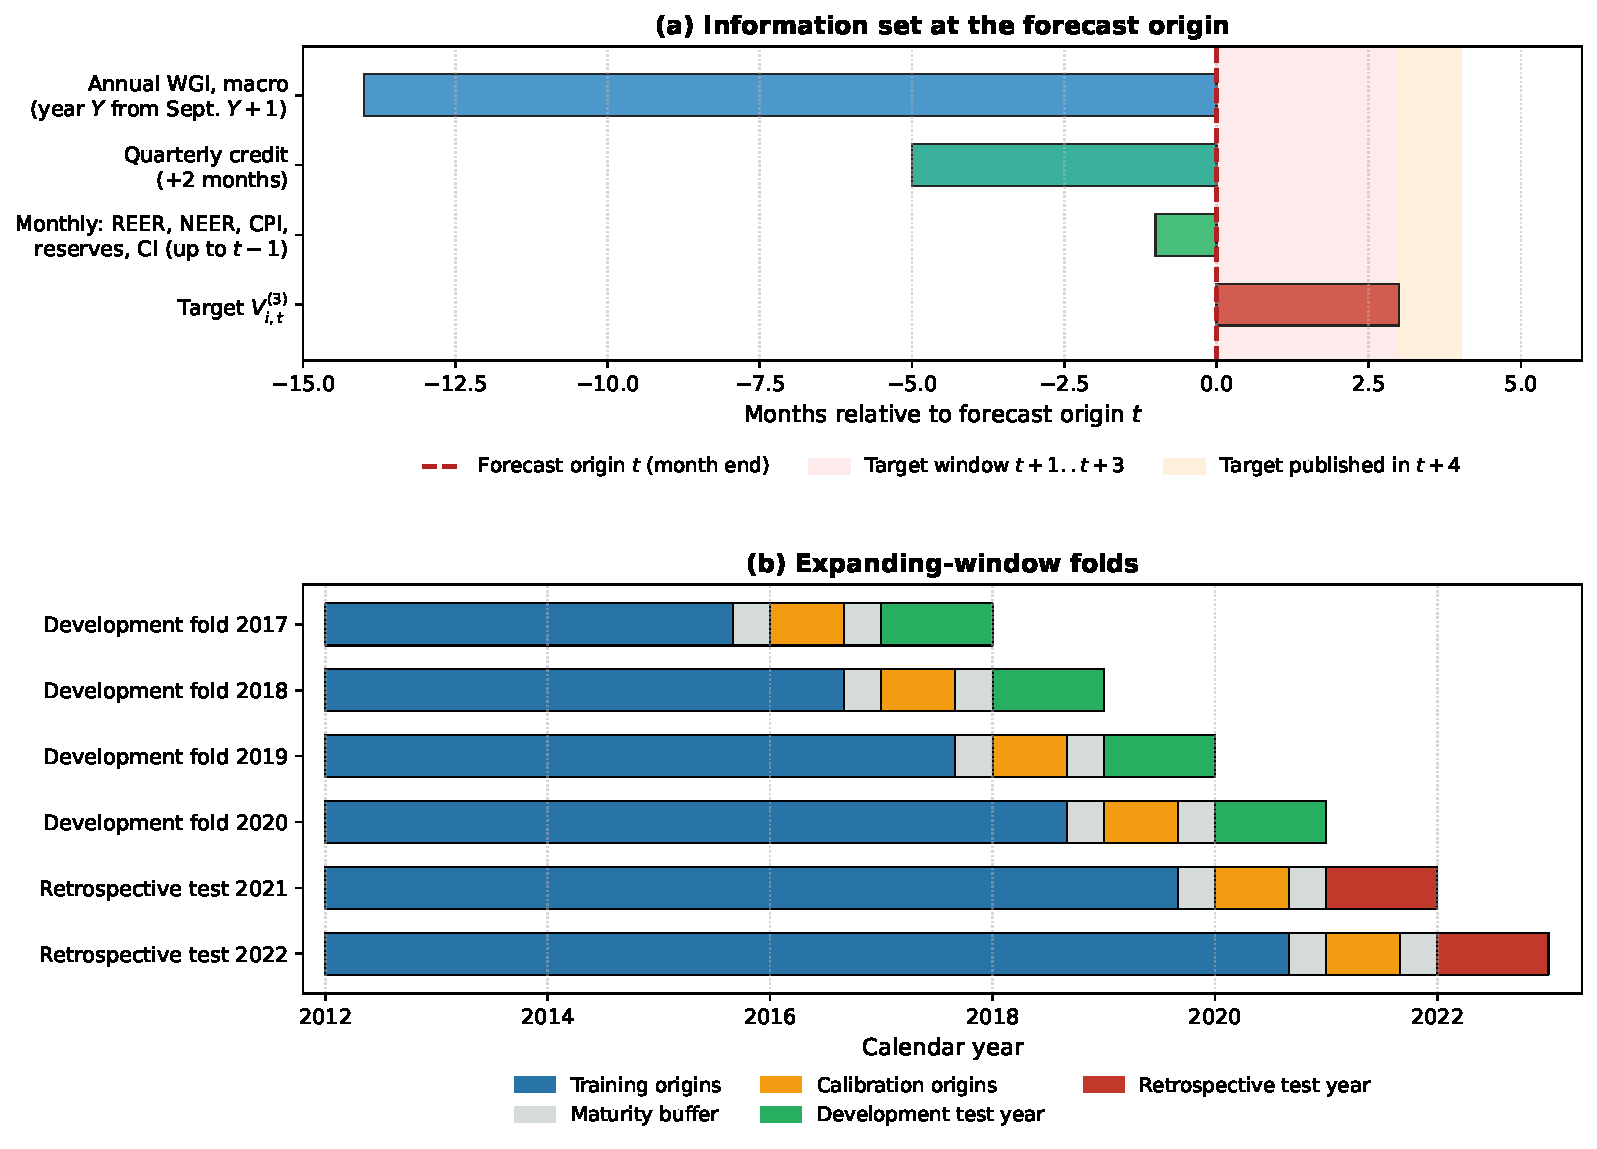
\includegraphics[width=\textwidth]{figures/Fig1.pdf}\caption{Information set at the forecast origin (a) and expanding-window folds (b).}\label{fig:fig1}\end{figure*}
\subsection{Targets and events}
The primary target is forward three-month REER stress,

\begin{equation}\label{eq:V}
V^{(3)}_{i,t} = \sqrt{\tfrac{1}{3}\left(r_{i,t+1}^2 + r_{i,t+2}^2 + r_{i,t+3}^2\right)}
\end{equation}
where $r_{i,t}$ is the monthly REER log change in percent. This root-mean-square measure captures large movements in either direction; it is not a demeaned volatility estimator or a dated currency-crisis label. Because consecutive windows share up to two months, high-risk windows overlap and are not independent events; inference therefore resamples blocks of months. A window is high-risk when $V^{(3)}_{i,t}$ is at or above the 80th percentile of the training targets of its fold; the thresholds range from 2.43\% to 2.69\%. Table~\ref{tab:folds} reports the samples and events of every fold: the development folds (2017-2020) contain 85 high-risk windows in 432 country-months and the retrospective test (2021-2022) 36 in 216 (10 in 2021 and 26 in 2022). A secondary target is the maximum three-month reserve drawdown, $D^{(3)}_{i,t} = \max\{0, 1 - \min_{k \le 3} R_{i,t+k}/R_{i,t}\}$. Scoring the main evaluation required outcome data up to 2023-04. An earlier data-availability audit computed target means through 2024-03; no model prediction for origins after 2022-12 was scored before the extension protocol was frozen. Fig.~\ref{fig:fig2} shows the stress windows and IQ trajectories.

The results presented below focus on the REER target. A reserve-drawdown definition alone does not provide evidence that the findings transfer to reserve pressure. Likewise, positive forecasting windows and the underlying economic episodes are different counting units.

\begin{table*}[!htbp]
\centering
\scriptsize
\setlength{\tabcolsep}{3pt}
\caption{Folds, samples and events (Core-9, h = 3).}
\label{tab:folds}
\begin{adjustbox}{max width=\textwidth}
\begin{tabular}{lllrrrrrr}
\toprule
Fold & Role & Threshold \% & Train origins & N train (pos.) & Calibration (pos.) & N test & Test pos. & Episodes \\
\midrule
2017 & development & 2.43 & 2012-01 to 2015-08 & 396 (80) & 72 (23) & 108 & 18 & 6 \\
2018 & development & 2.65 & 2012-01 to 2016-08 & 504 (101) & 72 (9) & 108 & 25 & 7 \\
2019 & development & 2.63 & 2012-01 to 2017-08 & 612 (123) & 72 (22) & 108 & 8 & 6 \\
2020 & development & 2.69 & 2012-01 to 2018-08 & 720 (144) & 72 (4) & 108 & 34 & 5 \\
2021 & retrospective & 2.57 & 2012-01 to 2019-08 & 828 (166) & 72 (29) & 108 & 10 & 5 \\
2022 & retrospective & 2.63 & 2012-01 to 2020-08 & 936 (188) & 72 (6) & 108 & 26 & 5 \\
\bottomrule
\end{tabular}
\end{adjustbox}
\par\vspace{2pt}\parbox{0.95\linewidth}{\scriptsize Note: Thresholds are the 80th percentile of the training targets of each fold. Training origins are truncated so that every target is published before the test year; the h = 6 task uses earlier cut-offs (Supplementary Table S16). Positives by country are listed in the replication package.}
\end{table*}
\begin{figure*}[!htbp]\centering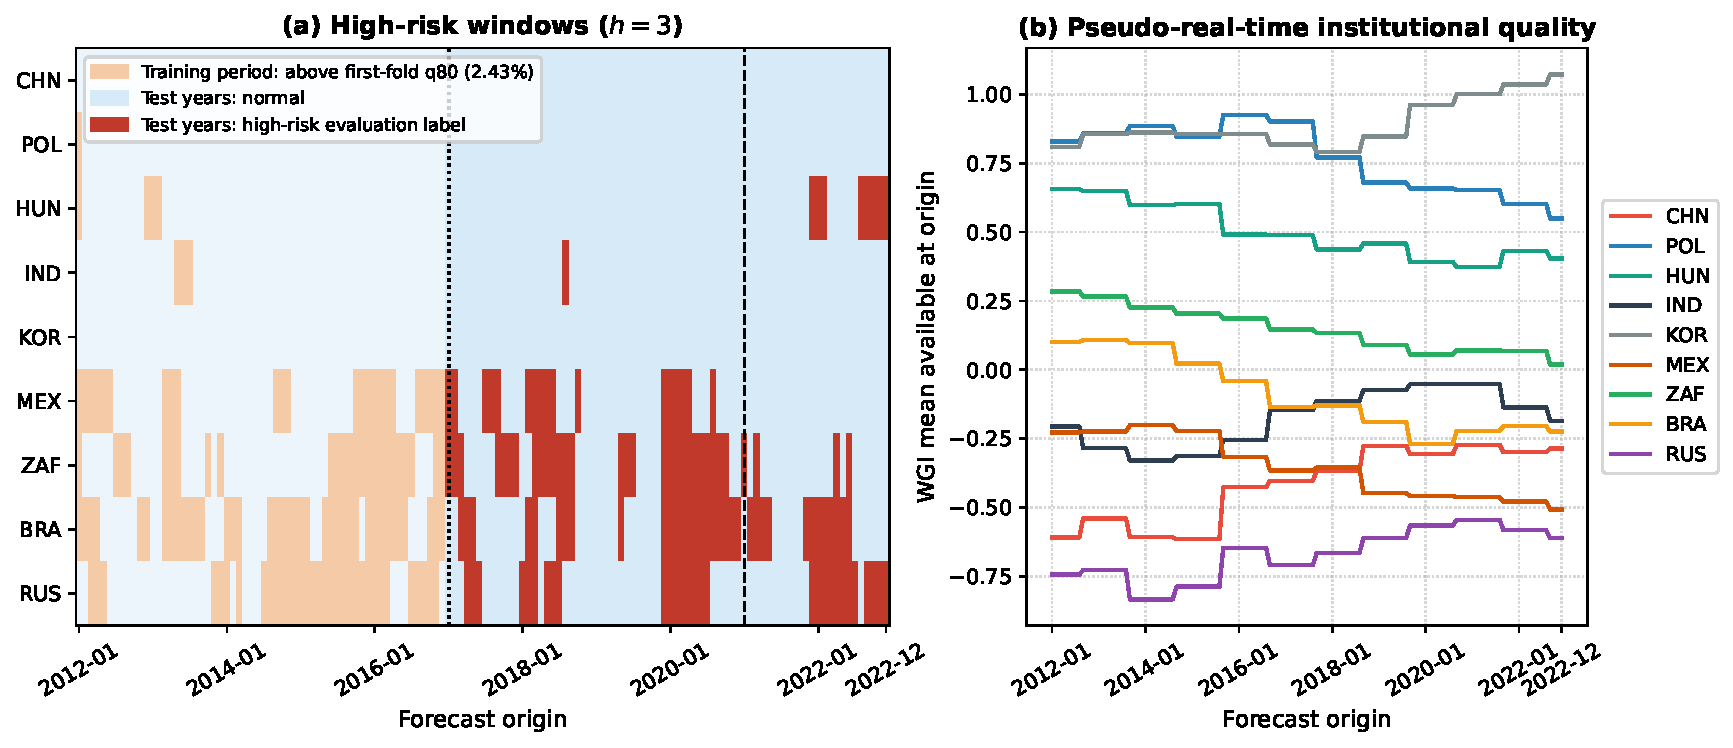
\includegraphics[width=\textwidth]{figures/Fig2.pdf}\caption{High-risk windows in the Core-9 panel (a) and pseudo-real-time institutional quality (b). In the test years the evaluation labels of each fold are shown; before 2017 the first-fold threshold is used for illustration.}\label{fig:fig2}\end{figure*}
\section{Forecasting and decision framework}
\subsection{System architecture}
The framework runs as scripts in a fixed order. (i) An information-timing module applies each publication lag, holds the last release forward and records data age. (ii) A replication auditor re-estimates the reported regressions and classifies each discrepancy as a convention, a suspected transcription error or a non-reproduction. (iii) A forecasting module fits all models on frozen splits and writes row-level predictions to a single prediction store. (iv) A decision module converts probabilities into alerts, review decisions and fallback choices. An audit script recomputes every reported metric from the prediction store, checks the timing of every estimation stage and blocks the manuscript build on any mismatch. Such checks complement, rather than replace, validation of the target, information set and estimation protocol.

\subsection{Temporal protocol}
Four expanding development folds test the years 2017-2020 and two retrospective folds test 2021 and 2022. In fold $T$, training origins run from 2012-01 to August of $T-2$, calibration origins from January to August of $T-1$ and test origins over year $T$. Every origin $s$ used for fitting or calibration satisfies

\begin{equation}\label{eq:mat}
s + h + \ell < \text{first evaluated month}
\end{equation}
with horizon $h$ and REER release lag $\ell = 1$, so every target used before an evaluation was published before it. The calendar cut-offs in Table~\ref{tab:folds} describe the three-month task; for $h = 6$ the training and calibration ranges are truncated further. The same condition is imposed inside the training window: hyperparameters are chosen by AP on three inner expanding folds (grids in Supplementary Table S13), each inner training range ends at least $h + \ell$ months before its validation range, and imputation and scaling are fitted on the inner training range only. Thresholds are estimated on the training targets of each outer fold. Supplementary Table S16 lists, for every fold, horizon and stage (outer training, calibration, inner folds and the calibration history described below), the last origin used, the month its target was published and the first evaluated month; all 102 stage checks of the main evaluation and of the post-hoc rerun in Section 5.9 pass. Development-fold performance is used for selection and should not be interpreted as an untouched test estimate.

\subsection{Models}
B0 is a persistence rule, a one-variable logistic map from the lagged three-month REER volatility. B1 is ridge regression for the continuous target and L2-regularised logistic regression for the binary target. B2 is a threshold forecaster that estimates an IQ threshold in the training window and fits regime-specific CI slopes. B3 and B4 are a random forest and XGBoost. M0 is an additive EBM, and M1 adds a single CI $\times$ IQ pairwise term, the forecasting analogue of the threshold hypothesis. Two country-identity baselines test whether learned models merely recognise countries: C0 is a logistic regression on country indicators and C1 adds the lagged REER volatility. The interaction ablation adds a placebo EBM with a macro-only pair, an unrestricted EBM with ten selected pairs and a linear CI $\times$ IQ model. Stochastic learners are averaged over five seeds.

\subsection{Calibration}
Each model produces raw probabilities and two calibrated versions: Platt scaling on the eight-month calibration window, and Platt scaling on all earlier out-of-sample predictions whose targets had matured ('expanding'). Because the event threshold changes from fold to fold, the expanding history is relabelled with the current fold's threshold before the Platt map is fitted, so that every pooled prediction refers to the event being forecast. For each model the scheme with the lowest pooled Brier score on the development folds is designated as the development-selected scheme; it was raw for 6 of the 7 models. All decision analyses use these probabilities. Because the 2021-2022 period had already been inspected during study design, its estimates are retrospective even when this calibration rule is held fixed.

\subsection{Code corrections after the first draft}
An internal code audit after the first draft found two departures from the protocol above. The inner tuning folds used a fixed gap of three months, shorter than the $h + \ell$ months required (four for $h = 3$, seven for $h = 6$), and the imputer and scaler were fitted on the whole training window before the inner split. In addition, the expanding calibration history kept each earlier fold's own event threshold. Both issues were corrected and every learned-model experiment was rerun; the earlier outputs are archived in the replication package. Of 766 audited numbers, 452 changed; the largest change in a headline pooled AP is 0.023, and the persistence and country-identity baselines are unchanged. Two conclusions of the first draft changed: the CI $\times$ IQ interaction is no longer equivalent to the additive model in 2021-2022 (90\% interval [-0.010, 0.037], previously [-0.005, 0.009]), and the random forest's gain over B0 is no longer distinguishable from zero (0.043 [-0.029, 0.176], previously 0.066 [0.001, 0.187]). The frozen 2023-2025 extension (Section 4.9) had already been scored with the earlier tuning code and was not rescored; its inner tuning folds fail the timing check (15 stage checks), and Section 5.9 reports a post-hoc rerun with the corrected code.

\subsection{Metrics and inference}
Average precision summarises the precision-recall curve,

\begin{equation}\label{eq:ap}
\mathrm{AP} = \sum_{k} (R_k - R_{k-1})\, P_k
\end{equation}
where $P_k$ and $R_k$ are precision and recall at the $k$-th threshold. We report pooled AP over all predictions of a window and the mean of the fold-specific APs; tables state which is shown. Alerts are issued when the probability $p$ reaches $\tau = C_{FP}/(C_{FP} + C_{FN})$, and the expected cost per 100 forecasts is

\begin{equation}\label{eq:cost}
\mathrm{Cost} = \frac{100}{n} \sum_{i} \left[ C_{FP}\, \mathbf{1}(p_i \ge \tau,\, y_i = 0) + C_{FN}\, \mathbf{1}(p_i < \tau,\, y_i = 1) \right]
\end{equation}
with $C_{FP} = 1$ and $C_{FN} = 5$ unless stated. Paired differences are assessed with a moving-block bootstrap that resamples calendar months jointly across countries (1,000 replications) \citep{kunsch1989}. We use blocks of 12 months for the 72-month window and of 6 months for 24- and 36-month windows, because a 24-month window contains only 13 distinct 12-month blocks; results for other lengths are in the replication package. We set the smallest effect of interest to $\Delta\mathrm{AP} = 0.02$, about a tenth of the typical gap between a skilled model and the base rate, and call two models equivalent when the 90\% interval lies within $\pm 0.02$, the two one-sided tests procedure \citep{schuirmann1987,lakens2017}.

The 0.02 margin is an operational tolerance for this comparison, not an externally validated economic utility threshold. Intervals are conditional on the fitted predictions and do not incorporate all uncertainty from model selection or refitting. Unless an adjustment is explicitly reported, the many model and sensitivity comparisons are exploratory. AP differences must be compared within matched samples because AP depends on event prevalence. The cost threshold of 1/6 is Bayes-optimal only when the probabilities are calibrated for the stated event and the assumed losses are appropriate.

\subsection{Event-level evaluation}
Consecutive high-risk origins of a country form an episode. Episode coverage counts an episode as covered when an alert is issued between three months before its first origin and its last origin. False alarms are alerts at normal origins outside the three months before an episode, per country-year. Because coverage permits alerts after an episode has started, it is not the fraction of episodes warned about in advance. We therefore add a strict early-warning measure: an episode is eligible when its three preceding origins are observed in the window, and it is detected only if an alert is issued at one of those three origins; the lead is the distance from the first such alert to the first high-risk origin. Besides the cost threshold $\tau$ we apply fixed alert quotas of the top one, two or three countries per month. Leads are relative to the first labelled origin, not to an independently dated crisis. Onset evaluation removes origins whose lagged volatility already exceeds the fold threshold; it evaluates predictions conditional on the absence of elevated lagged volatility. The direction analysis splits high-risk windows by the sign of the three-month REER change (real depreciation versus appreciation).

\subsection{Decision layer}
The review experiment is a scenario simulation, not an observed workflow. Each month analysts review $k$ country cases; a reviewed case costs a fee $c$, and the remaining cases are decided automatically at $\tau = 1/6$. In the baseline grid a reviewed case is resolved correctly with probability one (an oracle bound) or 0.8, and every automated policy (never alert, B0, macro-only EBM, M0, M1 with each calibration, B3, B4) is crossed with four routing rules: least confident first (smallest $|\mathrm{logit}\,p - \mathrm{logit}\,\tau|$, the distance to the cost-sensitive boundary rather than to 0.5), highest probability first, highest lagged volatility first and random. Random routing is evaluated as its exact expectation, so no simulation seed is involved.

A single accuracy does not determine the expected loss, so a second grid varies the reviewer-error model: errors independent of class with accuracy 0.8; more missed events (error rate 0.3 on events, 0.1 on non-events); more false alarms (0.1 and 0.3); and confidence-dependent errors that reach 0.4 at the decision boundary and decline with the logit distance from it. Errors are independent of country, and an error turns a reviewed case into the wrong decision. This grid adds expected-loss routing, which reviews the $k$ cases with the largest model-implied reduction in expected loss, $\mathrm{EL}_{auto} - \mathrm{EL}_{review}$, computed from the model probability and the same error model, and only when that reduction is positive. The rule uses no outcome information. Perfect review is an oracle bound, the imperfect-reviewer models are assumptions, and neither is evidence of observed human forecasting performance. Cost differences carry paired block-bootstrap intervals.

\subsection{Frozen protocol for the retrospective extension}
Before scoring model predictions in the 2023-2025 extension, we recorded a frozen protocol (SHA-256 910490582b8d...) that fixes the sample (Core-9 and External-6), the features (macro and IQ; no updated post-2022 CI observations are available), the folds (test years 2023-2025, with 2021-2022 as warm-up folds), the models (B0, B1, macro EBM and XGBoost), raw probabilities, the costs and a fallback policy. All models are trained on the pooled 15-country history, so External-6 is evaluated out of time but is not an unseen-country transfer (Supplementary Table S17). The policy deploys the learned model, chosen on the development folds as the macro EBM, in year $T$ only if, on the latest twelve matured origins, its AP exceeds that of B0 by at least $\delta = 0.02$ and its expected calibration error is at most 0.11 (the largest per-fold ECE of B0 in the development folds); otherwise it deploys B0. Applied once to the retrospective folds, the rule chose 2021: B0; 2022: B0. A post-freeze change to the scoring script, needed to read the frozen file, is logged in the package; the protocol itself was not changed.

The hash identifies the protocol file but does not independently establish when it was fixed. The extension is not described as a prospective or independently preregistered trial; the earlier target-summary audit and the post-freeze code change form part of its analysis history. After the code corrections in Section 4.5 we added a post-hoc rerun of the same folds that is explicitly exploratory: it refits B0, C1, B1, the macro-only and macro+IQ EBMs and the macro-only and macro+IQ XGBoost models with the corrected tuning, estimates the paired IQ increment, compares always-on policies with the frozen fallback, reports the yearly inputs of the fallback rule and evaluates a multi-candidate monitor that deploys whichever candidate has the largest recent AP gain over B0 subject to the frozen $\delta$ and ECE cap. The monitor was defined after the frozen result was known and is a new policy, not part of the protocol.

\section{Results}
\subsection{Replication of the threshold evidence}
Table~\ref{tab:thresh} compares the replicated threshold tests with the reported values. With Hansen's residual variance the replicated F statistics exceed the reported ones by a factor determined by the panel dimensions: reported/replicated = 0.841 in all six Panel A regressions, 0.896 in the five nine-country Panel B regressions and 0.882 in the eight-country Panel B ER\_Vol regression. Dividing instead by $T(N-1)$ reproduces 12 of the 12 reported F statistics to two decimals, which identifies a compatible convention without recovering the unavailable original code. 10 of 12 thresholds are reproduced to four decimals. Of the 24 reported regime coefficients, 11 are reproduced in coefficient and t statistic, 3 in the coefficient only and 7 are not reproduced; 3 differ from our estimates only by a digit or a sign and are classified as suspected transcription errors, although we cannot rule out other causes without the original code (Supplementary Table S1).

\begin{table*}[!htbp]
\centering
\scriptsize
\setlength{\tabcolsep}{3pt}
\caption{Replication of the reported threshold tests (threshold variable: IQ).}
\label{tab:thresh}
\par\smallskip{\textit{Panel A. Reconstructed statistics}}\par\smallskip
\begin{adjustbox}{max width=\textwidth}
\begin{tabular}{llrrrrr}
\toprule
Panel & Risk & N & Reported F & Matched F, T(N-1) & Hansen F & p \\
\midrule
A & CPI\_Vol & 678 & 400.68 & 400.68 & 476.56 & 0.0005 \\
A & FX\_Vol & 678 & 54.62 & 54.62 & 64.97 & 0.0195 \\
A & CE\_Vol & 678 & 120.64 & 120.64 & 143.49 & 0.0180 \\
A & ER\_Vol & 678 & 27.24 & 27.24 & 32.40 & 0.8885 \\
A & CG\_Gap & 678 & 83.12 & 83.12 & 98.86 & 0.0375 \\
A & Unemp & 678 & 103.64 & 103.64 & 123.27 & 0.0005 \\
B & CPI\_Vol & 1188 & 276.57 & 276.57 & 308.79 & 0.0450 \\
B & FX\_Vol & 1188 & 79.31 & 79.31 & 88.55 & 0.0295 \\
B & CE\_Vol & 1188 & 219.67 & 219.67 & 245.25 & 0.0005 \\
B & ER\_Vol & 1056 & 104.28 & 104.28 & 118.28 & 0.0605 \\
B & CG\_Gap & 1188 & 34.61 & 34.61 & 38.64 & 0.6500 \\
B & Unemp & 1188 & 54.34 & 54.34 & 60.67 & 0.1325 \\
\bottomrule
\end{tabular}
\end{adjustbox}
\par\smallskip{\textit{Panel B. Threshold location and sensitivity}}\par\smallskip
\begin{adjustbox}{max width=\textwidth}
\begin{tabular}{llrrrrr}
\toprule
Panel & Risk & Reported threshold & Reconstructed threshold & Low regime \% & p 15\% trim & p lag adjusted \\
\midrule
A & CPI\_Vol & -0.7870 & -0.7870 & 1.8 & 0.8910 & 0.6190 \\
A & FX\_Vol & 0.4481 & 0.4481 & 68.4 & 0.0175 & 0.3830 \\
A & CE\_Vol & -0.7116 & -0.7116 & 7.8 & 0.1650 & 0.0720 \\
A & ER\_Vol & -0.4764 & -0.4764 & 22.7 & 0.8085 & 0.0600 \\
A & CG\_Gap & -0.3692 & -0.3692 & 33.3 & 0.0300 & 0.0125 \\
A & Unemp & 0.0240 & 0.0240 & 51.8 & 0.0005 & 0.6380 \\
B & CPI\_Vol & -0.2560 & -0.2560 & 35.4 & 0.0030 & 0.0310 \\
B & FX\_Vol & -0.7541 & -0.7870 & 1.0 & 0.1390 & 0.0135 \\
B & CE\_Vol & -0.7234 & -0.7116 & 5.1 & 0.1595 & 0.0005 \\
B & ER\_Vol & -0.7039 & -0.7039 & 8.0 & 0.7235 & 0.5365 \\
B & CG\_Gap & -0.1554 & -0.1554 & 44.4 & 0.4705 & 0.7400 \\
B & Unemp & -0.1416 & -0.1416 & 46.5 & 0.0630 & 0.4970 \\
\bottomrule
\end{tabular}
\end{adjustbox}
\par\vspace{2pt}\parbox{0.95\linewidth}{\scriptsize Note: p-values from 1999 country-block residual bootstraps under the linear null, (1 + k)/(B + 1). Main specification: 1\% trimming, contemporaneous other risks.}
\end{table*}
\subsection{How robust are the thresholds?}
The thresholds are often extreme. In 5 of 12 regressions fewer than 10\% of observations fall in the low-IQ regime; for Panel A CPI\_Vol the low regime contains 1.8\% of observations. With 1\% trimming 8 of 12 tests are significant at 5\%; with 15\% trimming 4 of these lose significance (Panel A CPI\_Vol: p = 0.891), leaving Panel A FX\_Vol, Panel A CG\_Gap, Panel A Unemp, Panel B CPI\_Vol. In a pseudo-real-time version that lags CI by one month and uses IQ and annual controls only after their release, 4 tests are significant and 4 of the originally significant ones survive (Panel A CG\_Gap, Panel B CPI\_Vol, Panel B FX\_Vol, Panel B CE\_Vol). With single WGI dimensions as threshold variables, 6 of 36 Panel A and 9 of 36 Panel B tests are significant (Supplementary Tables S3-S5). Fig.~\ref{fig:fig8} summarises the evidence. The answer to RQ1 is that the threshold evidence is reproducible as computed but sensitive to specification and insufficient, on its own, to establish a stable predictive or causal mechanism.

\begin{figure*}[!htbp]\centering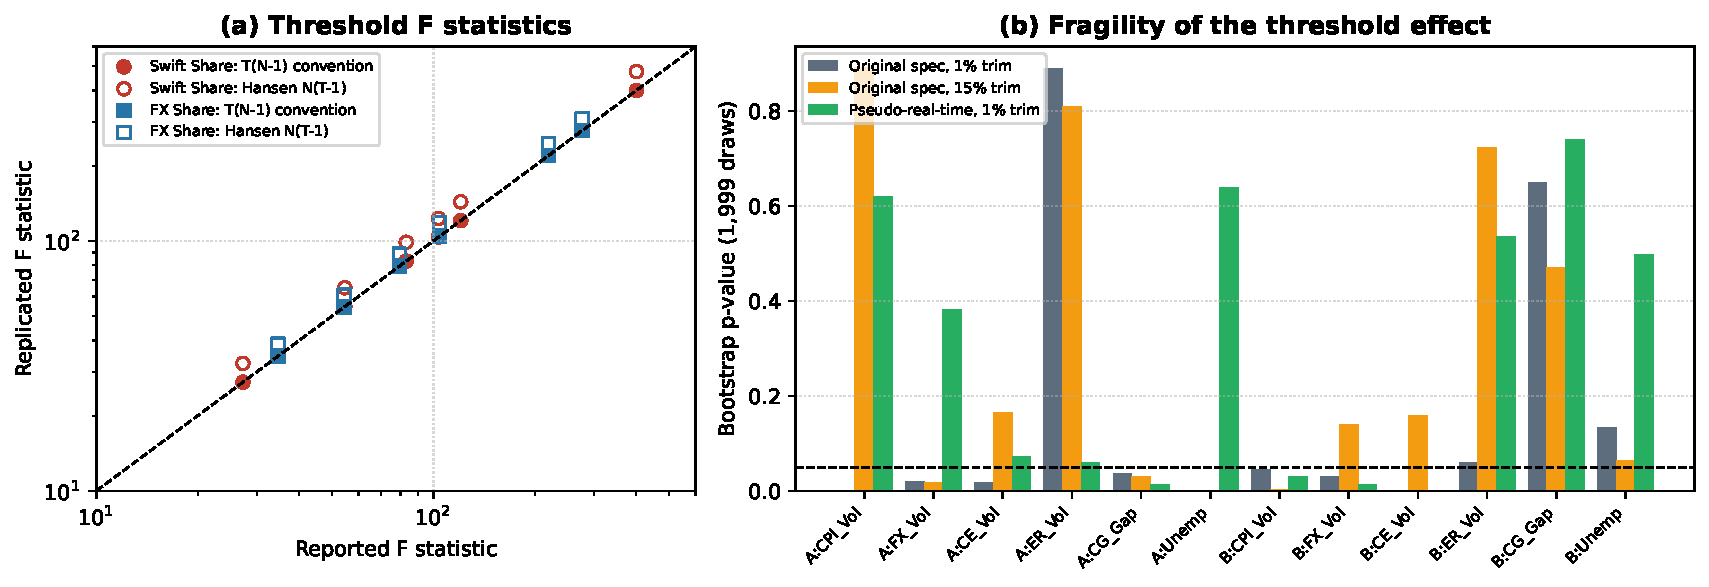
\includegraphics[width=\textwidth]{figures/Fig3.pdf}\caption{Replicated versus reported threshold F statistics (a) and bootstrap p-values under 1\% trimming, 15\% trimming and the pseudo-real-time specification (b).}\label{fig:fig8}\end{figure*}
\subsection{Forecasting benchmark}
Table~\ref{tab:bench} reports the benchmark. Over all six folds (pooled AP, base rate 0.187) the random forest leads with 0.483, followed by C1 (0.471), XGBoost (0.450) and the persistence rule B0 (0.440); the EBMs reach 0.388 (M0) and 0.382 (M1). The ranking is not stable. In the development folds the random forest is best (0.519) and B0 weak (0.405); in the retrospective test C1 reaches 0.574 and B0 0.535, above the other multivariable models in Table~\ref{tab:bench} (at most 0.478), and the EBMs fall to about 0.322. Paired bootstrap intervals over the six folds show no AP gain over B0 whose lower 95\% limit exceeds zero: the random forest's gain is 0.043 [-0.029, 0.176] and XGBoost's 0.010 [-0.035, 0.128]. Country identity alone (C0) reaches 0.378, close to the EBMs, which is consistent with cross-country differences contributing to discrimination, without quantifying how much of each model's skill is attributable to country identity (Fig.~\ref{fig:fig3}).

\begin{table}[!htbp]
\centering
\scriptsize
\setlength{\tabcolsep}{3pt}
\caption{Forecasting benchmark for three-month REER stress (Core-9).}
\label{tab:bench}
\par\smallskip{\textit{Panel A. Ranking performance}}\par\smallskip
\begin{adjustbox}{max width=\textwidth}
\begin{tabular}{llrrrr}
\toprule
Model & AP all pooled & AP all mean & AP dev pooled & AP retro pooled & AP retro mean \\
\midrule
B0 Persistence & 0.440 & 0.377 & 0.405 & 0.535 & 0.475 \\
C0 Country identity & 0.378 & 0.434 &  & 0.480 & 0.474 \\
C1 Country + persistence & 0.471 & 0.436 &  & 0.574 & 0.531 \\
B1 Ridge / logistic & 0.380 & 0.410 & 0.447 & 0.354 & 0.387 \\
B2 Threshold model & 0.386 & 0.466 & 0.422 & 0.362 & 0.396 \\
B3 Random forest & 0.483 & 0.421 & 0.519 & 0.478 & 0.385 \\
B4 XGBoost & 0.450 & 0.412 & 0.506 & 0.421 & 0.370 \\
M0 EBM additive & 0.388 & 0.410 & 0.476 & 0.317 & 0.360 \\
M1 EBM + CI $\times$ IQ & 0.382 & 0.410 & 0.439 & 0.322 & 0.380 \\
\bottomrule
\end{tabular}
\end{adjustbox}
\par\smallskip{\textit{Panel B. Retrospective probability and cost performance}}\par\smallskip
\begin{adjustbox}{max width=\textwidth}
\begin{tabular}{llrr}
\toprule
Model & Brier retro & Cost retro & Calibration \\
\midrule
B0 Persistence & 0.111 & 41.2 & raw \\
C0 Country identity & 0.126 & 50.0 & raw \\
C1 Country + persistence & 0.116 & 50.0 & raw \\
B1 Ridge / logistic & 0.182 & 52.3 & raw \\
B2 Threshold model & 0.138 & 52.3 & platt expanding \\
B3 Random forest & 0.121 & 49.1 & raw \\
B4 XGBoost & 0.121 & 49.5 & raw \\
M0 EBM additive & 0.147 & 66.7 & raw \\
M1 EBM + CI $\times$ IQ & 0.148 & 69.0 & raw \\
\bottomrule
\end{tabular}
\end{adjustbox}
\par\vspace{2pt}\parbox{0.95\linewidth}{\scriptsize Note: 'all': six folds, 648 country-months, 121 positives; 'dev': 2017-2020; 'retro': 2021-2022, 216 country-months, 36 positives. Cost: expected cost per 100 forecasts at C\_FN = 5. Calibration: scheme selected on the development folds; C0 and C1 calibration not selected separately (raw shown).}
\end{table}
\begin{figure*}[!htbp]\centering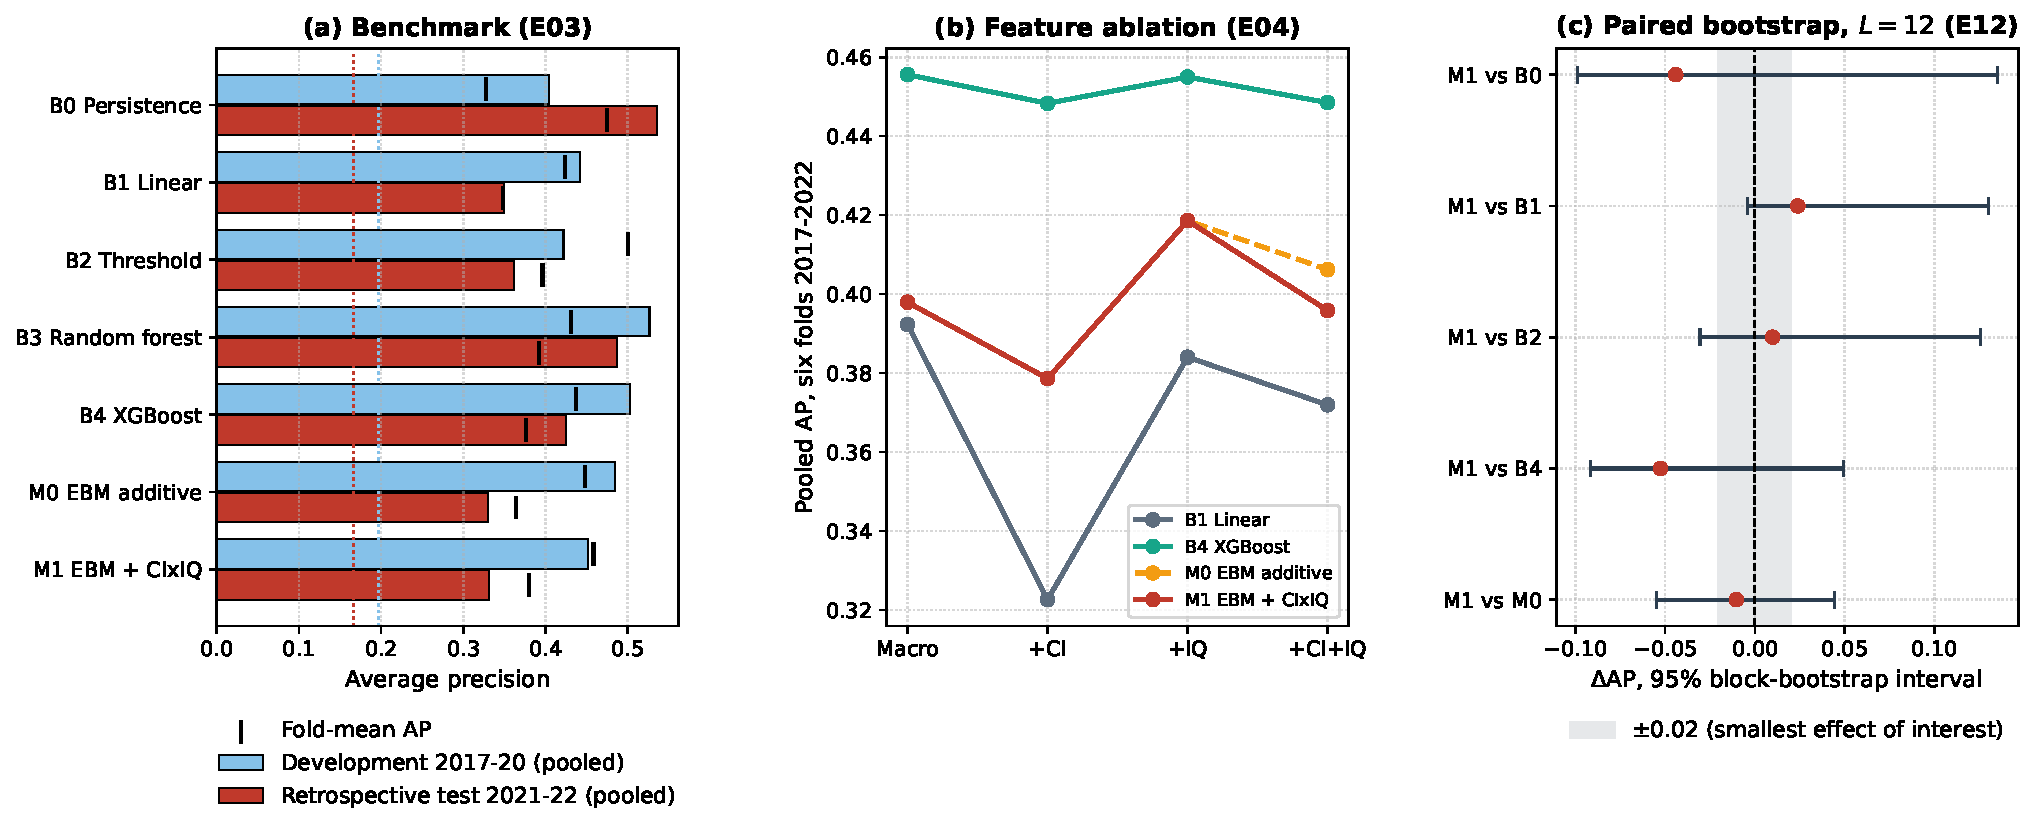
\includegraphics[width=\textwidth]{figures/Fig4.pdf}\caption{(a) Pooled AP in the development and retrospective folds with fold-mean AP marked; dotted lines give the base rates. (b) Pooled AP over six folds by feature set. (c) Paired block-bootstrap intervals (L = 12) for M1 against each benchmark over six folds; the shaded band is the smallest effect of interest.}\label{fig:fig3}\end{figure*}
\subsection{Do CI and IQ add information?}
Table~\ref{tab:ablation} compares CI and IQ additions in the main FX-share specification. Adding CI to the macro feature set lowers pooled AP in 5 of 6 model-window cells, and no addition of CI, IQ or both raises AP by 0.02 or more in any of 18 cells. Relative to M0, the CI $\times$ IQ interaction changes AP by -0.006 over all folds and +0.005 in the retrospective test, a placebo macro interaction by +0.003 and +0.005, and an unrestricted EBM by +0.022 and -0.006. The paired bootstrap gives M1 minus M0 = -0.005 [-0.029, 0.021] over six folds and 0.005 [-0.013, 0.040] in the retrospective test. Neither 90\% interval ([-0.024, 0.017] and [-0.010, 0.037]) lies within $\pm 0.02$, so equivalence is not established in either window.

\begin{table}[!htbp]
\centering
\scriptsize
\setlength{\tabcolsep}{3pt}
\caption{Contribution of CI, IQ and interactions (pooled AP).}
\label{tab:ablation}
\par\smallskip{\textit{Panel A. All six folds}}\par\smallskip
\begin{adjustbox}{max width=\textwidth}
\begin{tabular}{llrrr}
\toprule
Model or specification & Macro or model AP & Delta +CI & Delta +IQ & Delta +CI+IQ or vs M0 \\
\midrule
B1 Ridge / logistic & 0.391 & -0.008 & -0.008 & -0.010 \\
B4 XGBoost & 0.457 & -0.007 & -0.003 & -0.007 \\
M0 EBM additive & 0.395 & -0.020 & -0.004 & -0.007 \\
M1 CI $\times$ IQ pair vs M0 & 0.382 &  &  & -0.006 \\
Placebo macro pair vs M0 & 0.391 &  &  & +0.003 \\
Unrestricted EBM vs M0 & 0.410 &  &  & +0.022 \\
Linear CI $\times$ IQ vs M0 & 0.360 &  &  & -0.028 \\
\bottomrule
\end{tabular}
\end{adjustbox}
\par\smallskip{\textit{Panel B. Retrospective folds}}\par\smallskip
\begin{adjustbox}{max width=\textwidth}
\begin{tabular}{llrrr}
\toprule
Model or specification & Macro or model AP & Delta +CI & Delta +IQ & Delta +CI+IQ or vs M0 \\
\midrule
B1 Ridge / logistic & 0.366 & +0.004 & -0.049 & -0.012 \\
B4 XGBoost & 0.440 & -0.023 & -0.012 & -0.018 \\
M0 EBM additive & 0.340 & -0.023 & +0.007 & -0.022 \\
M1 CI $\times$ IQ pair vs M0 & 0.322 &  &  & +0.005 \\
Placebo macro pair vs M0 & 0.323 &  &  & +0.005 \\
Unrestricted EBM vs M0 & 0.312 &  &  & -0.006 \\
Linear CI $\times$ IQ vs M0 & 0.331 &  &  & +0.014 \\
\bottomrule
\end{tabular}
\end{adjustbox}
\par\vspace{2pt}\parbox{0.95\linewidth}{\scriptsize Note: Upper rows: AP of the macro-only set and changes from adding CI, IQ or both. Lower rows: AP of the interaction specification and change relative to M0 with all features. Paired block bootstrap for M1 minus M0: six folds -0.005 [-0.029, 0.021] (L = 12); retrospective 0.005 [-0.013, 0.040] (L = 6). Smallest effect of interest: 0.02.}
\end{table}
Point estimates below 0.02 do not show that the underlying effects are below 0.02. Table~\ref{tab:intervals} therefore gives paired intervals for all 18 increments. In 9 of 18 the 95\% interval excludes a gain of 0.02 and in 4 the 90\% interval lies within $\pm 0.02$; the remaining 9 intervals, mostly for IQ and for the 24-month retrospective window, reach upper limits of up to 0.073, so a gain of that size cannot be excluded there. Only 1 interval excludes zero, a loss from adding IQ to B1 in 2021-2022 (-0.049 [-0.069, -0.018]). The evidence is therefore an absence of detected gains with limited precision, not a demonstrated absence of value.

\begin{table*}[!htbp]
\centering
\scriptsize
\setlength{\tabcolsep}{3pt}
\caption{Paired intervals for the feature-set increments of Table 5 (Delta AP relative to the macro-only set).}
\label{tab:intervals}
\begin{adjustbox}{max width=\textwidth}
\begin{tabular}{lllrrrrr}
\toprule
Model & Increment & All folds Delta [95\% CI] & Excl. +0.02 & TOST & Retro Delta [95\% CI] & Excl. +0.02 & TOST \\
\midrule
B1 Ridge / logistic & +CI & -0.008 [-0.065, 0.011] & yes & no & +0.004 [-0.022, 0.033] & no & no \\
B1 Ridge / logistic & +IQ & -0.008 [-0.023, 0.016] & yes & yes & -0.049 [-0.069, -0.018] & yes & no \\
B1 Ridge / logistic & +CI+IQ & -0.010 [-0.050, 0.022] & no & no & -0.012 [-0.055, 0.064] & no & no \\
B4 XGBoost & +CI & -0.007 [-0.018, 0.005] & yes & yes & -0.023 [-0.046, 0.025] & no & no \\
B4 XGBoost & +IQ & -0.003 [-0.012, 0.013] & yes & yes & -0.012 [-0.033, 0.008] & yes & no \\
B4 XGBoost & +CI+IQ & -0.007 [-0.018, 0.008] & yes & yes & -0.018 [-0.046, 0.022] & no & no \\
M0 EBM additive & +CI & -0.020 [-0.051, 0.007] & yes & no & -0.023 [-0.056, -0.000] & yes & no \\
M0 EBM additive & +IQ & -0.004 [-0.059, 0.028] & no & no & +0.007 [-0.034, 0.073] & no & no \\
M0 EBM additive & +CI+IQ & -0.007 [-0.027, 0.027] & no & no & -0.022 [-0.064, 0.058] & no & no \\
\bottomrule
\end{tabular}
\end{adjustbox}
\par\vspace{2pt}\parbox{0.95\linewidth}{\scriptsize Note: Moving-block bootstrap over months, 1,000 replications; L = 12 (all folds, 121 positives) and L = 6 (retrospective, 36 positives). 'Excl. +0.02': the 95\% interval lies below +0.02. 'TOST': the 90\% interval lies within +/-0.02. Intervals for the Core-6 CI measures and for every robustness specification are in the replication package (table16\_e21\_paired\_intervals.csv).}
\end{table*}
Why does the CI signal not help? The EBM explanations (Fig.~\ref{fig:fig5}) rank the FX share 4 of 24 terms and the CI $\times$ IQ pair 17; the CI response is almost parallel across IQ levels. Replacing the FX share level by an expanding country mean (between) and the deviation from it (within) moves M0's pooled AP from 0.388 to 0.410, compared with 0.395 for the macro-only M0; adding a within $\times$ IQ or a between $\times$ IQ pair gives 0.405 and 0.396. The between component carries 6.2\% of total EBM importance against 1.8\% for the within component (Supplementary Table S14). This decomposition is consistent with part of the CI signal reflecting persistent country differences; importance shares do not establish that CI is only a country identifier or identify a causal channel.

\begin{figure*}[!htbp]\centering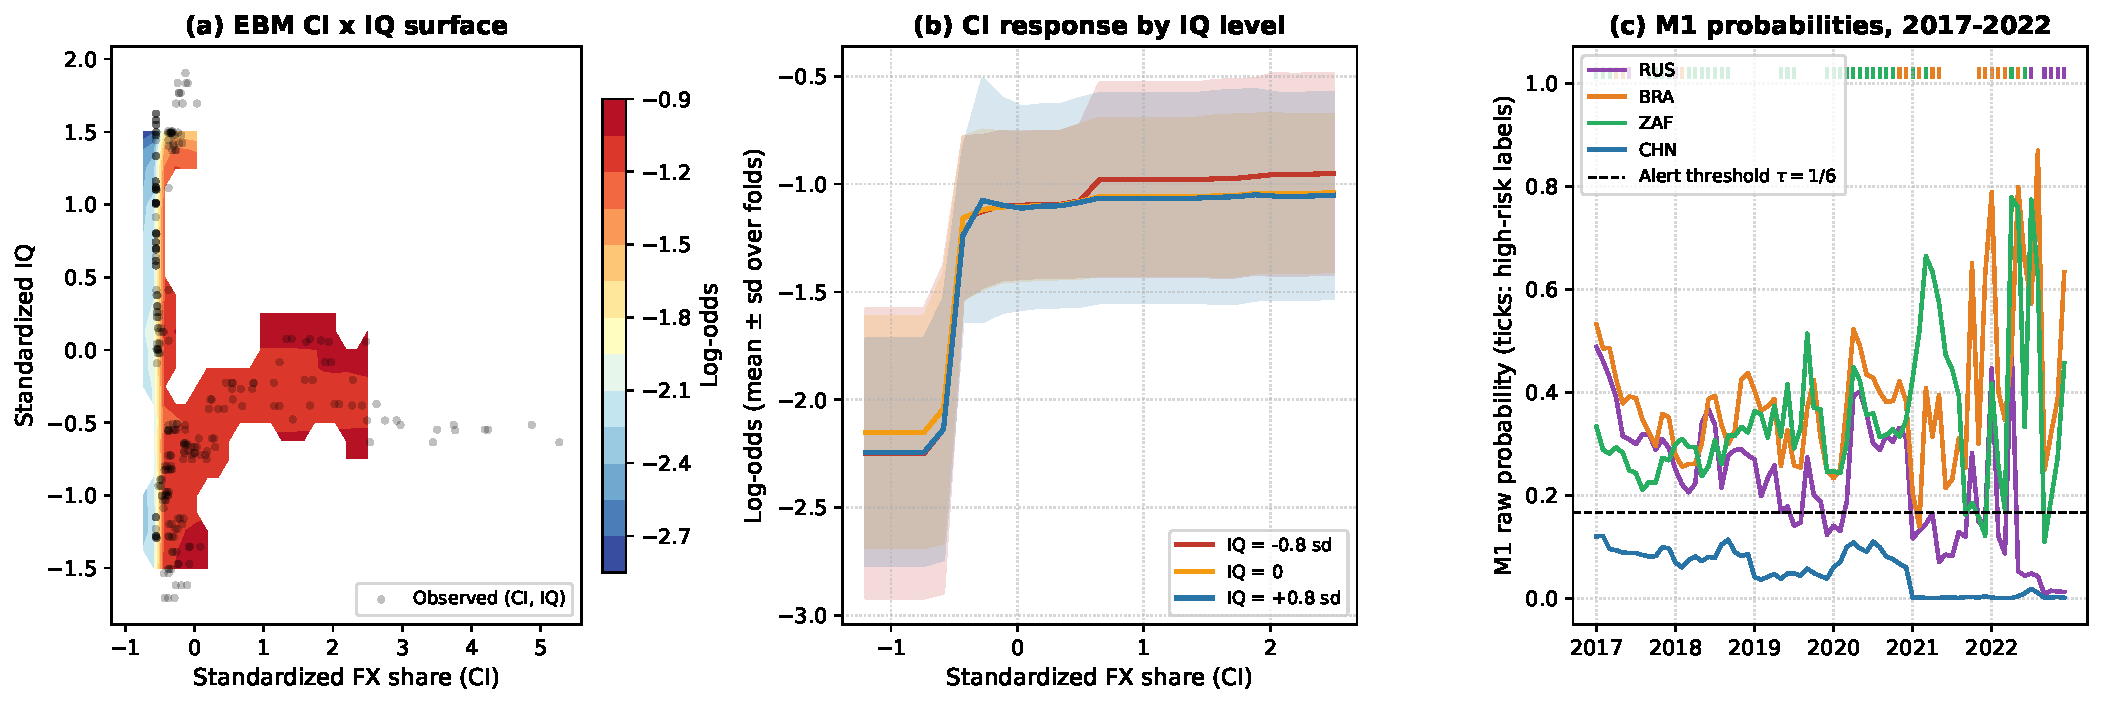
\includegraphics[width=\textwidth]{figures/Fig5.pdf}\caption{EBM CI $\times$ IQ surface with sparse cells masked (a), CI response at three IQ levels with fold variability (b) and raw M1 probabilities with high-risk labels for four countries (c).}\label{fig:fig5}\end{figure*}
\subsection{Events, onsets and direction}
Table~\ref{tab:events} moves from windows to episodes. Over six folds there are 31 episodes (10 in 2021-2022). At $C_{FN} = 5$, B0 covers 90\% of episodes with 2.17 false alarms per country-year, XGBoost 94\% with 2.07 and M1 87\% with 1.83; in the retrospective test M1 covers only 70\%. Under the strict definition, 28 episodes are eligible (7 in 2021-2022). B0 warns before the start of 82\% of them, XGBoost 89\%, C1 89\% and M1 86\%, with a median lead of 3.0 months, the maximum the definition allows; in 2021-2022 the shares are 86\%, 86\%, 71\% and 57\%. With a fixed quota of two countries per month, false alarms fall to below one per country-year, and B0 still detects 75\% of episodes in advance against 54\% for XGBoost and 68\% for M1. When origins already in stress are removed, AP falls for every model, and in the retrospective test C1 (0.509) still leads M1 (0.311) and B0 (0.295) in the onset-restricted sample (20 onset windows). Over six folds most models predict depreciation and appreciation windows with similar AP (B0 0.277 and 0.345, M1 0.236 and 0.256). In 2021-2022 the persistence-based models detect the 15 depreciation windows much better (B0 0.488, C1 0.511) than the EBMs (M1 0.193).

\begin{table*}[!htbp]
\centering
\scriptsize
\setlength{\tabcolsep}{3pt}
\caption{Episode coverage, strict early warning, onset and direction results.}
\label{tab:events}
\par\smallskip{\textit{Panel A. All six folds}}\par\smallskip
\begin{adjustbox}{max width=\textwidth}
\begin{tabular}{llrrrrrrr}
\toprule
Model & Episode coverage \% & False alarms / country-year & Strict detection \% (tau) & Strict detection \% (top-2) & False alarms (top-2) & Onset AP & Depr. AP & Appr. AP \\
\midrule
B0 Persistence & 90 & 2.17 & 82 & 75 & 0.87 & 0.217 & 0.277 & 0.345 \\
C1 Country + persistence & 90 & 2.06 & 89 & 68 & 0.81 & 0.306 & 0.323 & 0.331 \\
B1 Ridge / logistic & 94 & 1.80 & 93 & 61 & 0.87 & 0.365 & 0.223 & 0.266 \\
B3 Random forest & 94 & 2.59 & 89 & 61 & 0.91 & 0.302 & 0.347 & 0.322 \\
B4 XGBoost & 94 & 2.07 & 89 & 54 & 0.85 & 0.361 & 0.299 & 0.308 \\
M0 EBM additive & 87 & 1.74 & 86 & 68 & 0.93 & 0.328 & 0.243 & 0.255 \\
M1 EBM + CI $\times$ IQ & 87 & 1.83 & 86 & 68 & 0.93 & 0.331 & 0.236 & 0.256 \\
\bottomrule
\end{tabular}
\end{adjustbox}
\par\smallskip{\textit{Panel B. Retrospective folds}}\par\smallskip
\begin{adjustbox}{max width=\textwidth}
\begin{tabular}{llrrrrrrr}
\toprule
Model & Episode coverage \% & False alarms / country-year & Strict detection \% (tau) & Strict detection \% (top-2) & False alarms (top-2) & Onset AP & Depr. AP & Appr. AP \\
\midrule
B0 Persistence & 90 & 2.94 & 86 & 71 & 0.94 & 0.295 & 0.488 & 0.357 \\
C1 Country + persistence & 80 & 3.06 & 71 & 57 & 0.94 & 0.509 & 0.511 & 0.401 \\
B1 Ridge / logistic & 90 & 2.83 & 86 & 57 & 1.22 & 0.445 & 0.203 & 0.264 \\
B3 Random forest & 90 & 4.22 & 86 & 43 & 1.50 & 0.297 & 0.458 & 0.285 \\
B4 XGBoost & 90 & 2.89 & 86 & 43 & 1.39 & 0.320 & 0.299 & 0.294 \\
M0 EBM additive & 70 & 2.22 & 57 & 43 & 1.67 & 0.277 & 0.179 & 0.234 \\
M1 EBM + CI $\times$ IQ & 70 & 2.44 & 57 & 43 & 1.67 & 0.311 & 0.193 & 0.237 \\
\bottomrule
\end{tabular}
\end{adjustbox}
\par\vspace{2pt}\parbox{0.95\linewidth}{\scriptsize Note: Coverage and the first false-alarm column use alerts at tau = 1/6 and count alerts issued up to the end of an episode. Strict detection: share of eligible episodes (28 all folds, 7 retrospective) with an alert in the three origins before the first high-risk origin, at tau = 1/6 or with the top two countries per month. Episodes: 31 (all folds), 10 (2021-2022). Onset windows: 67 (all), 20 (retro). Lead-time distributions and top-1/top-3 quotas are in the replication package.}
\end{table*}
\subsection{Calibration and the decision layer}
Platt scaling on the eight-month window worsens the pooled Brier score for 7 of 7 models (M1: 0.133 raw, 0.202 with eight-month Platt, 0.144 with expanding Platt); calibration windows contain as few as 4 events. In the automated setting M1 costs 44.1 per 100 forecasts against 53.4 for B0 over six folds (difference -9.3 [-36.0, 6.5]), and 69.0 against 41.2 in the retrospective test (27.8 [2.3, 41.2]; Fig.~\ref{fig:fig4}). Table~\ref{tab:review} reports the review simulation with two reviews per month and a fee of 0.5. Routing the least confident M1 cases beats random routing in both windows (-6.9 [-14.5, -2.1] and -10.1 [-19.1, -2.7]), and oracle review also helps B0 (-6.5 [-14.2, -0.3]). Whether M1 with review beats B0 with review depends on the window: -8.3 [-31.2, 3.6] over six folds and 18.5 [-2.8, 34.3] in 2021-2022.

\begin{table*}[!htbp]
\centering
\scriptsize
\setlength{\tabcolsep}{3pt}
\caption{Selective-review scenario simulation: expected cost per 100 forecasts and paired differences.}
\label{tab:review}
\begin{adjustbox}{max width=\textwidth}
\begin{tabular}{lllrrrr}
\toprule
Period & Policy A & Policy B & Cost A & Cost B & A - B, accuracy 1.0 [95\% CI] & A - B, accuracy 0.8 [95\% CI] \\
\midrule
all & M1 + LC review & B0 + LC review & 38.6 & 46.9 & -8.3 [-31.2, 3.6] & -8.0 [-29.6, 3.1] \\
all & M1 + LC review & B0 automated & 38.6 & 53.4 & -14.8 [-42.4, -1.5] & -7.2 [-33.0, 5.1] \\
all & M1 + LC review & Never alert + vol. review & 38.6 & 60.5 & -21.9 [-49.4, -2.3] & -25.7 [-54.0, -6.2] \\
all & M1 + LC review & M1 + random review & 38.6 & 45.4 & -6.9 [-14.5, -2.1] & -7.0 [-14.1, -1.6] \\
all & M1 + LC review & Macro EBM + LC review & 38.6 & 36.7 & +1.9 [-6.2, 5.2] & +0.1 [-7.7, 3.7] \\
all & M1 automated & B0 automated & 44.1 & 53.4 & -9.3 [-36.0, 6.5] & -9.3 [-36.0, 6.5] \\
all & M1 Platt 8m automated & M1 raw automated & 71.8 & 44.1 & +27.6 [15.3, 57.6] & +27.6 [15.3, 57.6] \\
all & B0 + LC review & B0 automated & 46.9 & 53.4 & -6.5 [-14.2, -0.3] & +0.8 [-5.7, 5.9] \\
all & B0 + LC review & Never alert + vol. review & 46.9 & 60.5 & -13.6 [-23.8, 4.2] & -17.8 [-29.4, 0.4] \\
all & B0 automated & Never alert & 53.4 & 93.4 & -40.0 [-63.1, -13.9] & -40.0 [-63.1, -13.9] \\
retro & M1 + LC review & B0 + LC review & 54.6 & 36.1 & +18.5 [-2.8, 34.3] & +17.4 [-4.2, 32.4] \\
retro & M1 + LC review & B0 automated & 54.6 & 41.2 & +13.4 [-3.2, 24.5] & +20.8 [2.9, 31.9] \\
retro & M1 + LC review & Never alert + vol. review & 54.6 & 43.5 & +11.1 [-12.5, 26.4] & +5.9 [-18.5, 21.4] \\
retro & M1 + LC review & M1 + random review & 54.6 & 64.8 & -10.1 [-19.1, -2.7] & -10.1 [-18.8, -3.2] \\
retro & M1 + LC review & Macro EBM + LC review & 54.6 & 46.8 & +7.9 [-3.7, 18.5] & +6.4 [-4.6, 17.0] \\
retro & M1 automated & B0 automated & 69.0 & 41.2 & +27.8 [2.3, 41.2] & +27.8 [2.3, 41.2] \\
retro & M1 Platt 8m automated & M1 raw automated & 78.7 & 69.0 & +9.7 [3.2, 23.6] & +9.7 [3.2, 23.6] \\
retro & B0 + LC review & B0 automated & 36.1 & 41.2 & -5.1 [-15.7, 1.9] & +3.4 [-4.7, 8.5] \\
retro & B0 + LC review & Never alert + vol. review & 36.1 & 43.5 & -7.4 [-32.4, 12.0] & -11.5 [-36.5, 8.9] \\
retro & B0 automated & Never alert & 41.2 & 83.3 & -42.1 [-78.2, -5.6] & -42.1 [-78.2, -5.6] \\
\bottomrule
\end{tabular}
\end{adjustbox}
\par\vspace{2pt}\parbox{0.95\linewidth}{\scriptsize Note: LC review: least-confident cases (closest to the cost threshold) reviewed first; vol. review: highest lagged volatility first. Two reviews per month (k = 2), review fee 0.5, C\_FN = 5. M1 uses its development-selected calibration. Block bootstrap: L = 12 (all), L = 6 (retro). Accuracy 1.0 is an oracle bound. The full grid of policies, routing rules, budgets and fees is in the replication package.}
\end{table*}
Table~\ref{tab:reviewerr} varies the reviewer-error model. With perfect review, expected-loss routing beats low-confidence routing for B0 (-2.6 [-5.4, -0.8]) but not for M1 (4.1 [-2.6, 11.2]), and in 2021-2022 it is worse for M1 (11.3 [0.9, 20.6]), because the rule trusts probabilities that were poorly calibrated in that period. With any of the four imperfect-reviewer models and a fee of 0.5, the model-implied gain of review is never positive, so expected-loss routing reviews no case and equals no review in all 16 policy-error combinations. Low-confidence routing still beats random routing in 11 of 16 combinations, but it never significantly beats no review and is significantly worse in 3. The value of review therefore depends on reviewer accuracy, fees, calibration and the comparison policy; it is not a general property of the routing rule.

\begin{table}[!htbp]
\centering
\scriptsize
\setlength{\tabcolsep}{3pt}
\caption{Review routing under alternative reviewer-error models (all six folds; cost per 100 forecasts, A - B [95\% CI]).}
\label{tab:reviewerr}
\begin{tabular}{lllrr}
\toprule
Reviewer-error model & Automated policy & LC - random & Expected-loss - LC & LC - no review \\
\midrule
Perfect reviewer & B0 persistence & -5.7 [-11.0, -0.5] & -2.6 [-5.4, -0.8] & -6.5 [-14.2, -0.3] \\
Perfect reviewer & M1 EBM & -6.9 [-14.5, -2.1] & +4.1 [-2.6, 11.2] & -5.6 [-13.7, 2.3] \\
Perfect reviewer & Macro-only EBM & -6.0 [-9.3, -2.3] & +0.9 [-3.7, 4.5] & -3.9 [-9.0, 2.3] \\
Perfect reviewer & B4 XGBoost & -8.1 [-15.3, -2.7] & +0.2 [-3.5, 3.2] & -6.6 [-14.4, -0.8] \\
Symmetric, accuracy 0.8 & B0 persistence & -6.2 [-10.6, -1.9] & -0.8 [-5.9, 5.7] & +0.8 [-5.7, 5.9] \\
Symmetric, accuracy 0.8 & M1 EBM & -7.0 [-14.1, -1.6] & -2.1 [-10.1, 5.4] & +2.1 [-5.4, 10.1] \\
Symmetric, accuracy 0.8 & Macro-only EBM & -4.3 [-8.0, -0.1] & -5.5 [-12.3, -0.1] & +5.5 [0.1, 12.3] \\
Symmetric, accuracy 0.8 & B4 XGBoost & -7.5 [-14.2, -2.9] & -1.8 [-6.9, 5.1] & +1.8 [-5.1, 6.9] \\
Misses events more often (FN 0.3, FP 0.1) & B0 persistence & -6.6 [-10.4, -2.8] & -0.7 [-5.0, 5.2] & +0.7 [-5.2, 5.0] \\
Misses events more often (FN 0.3, FP 0.1) & M1 EBM & -7.1 [-13.7, -1.4] & -2.3 [-10.6, 4.9] & +2.3 [-4.9, 10.6] \\
Misses events more often (FN 0.3, FP 0.1) & Macro-only EBM & -3.1 [-7.4, 1.8] & -7.0 [-14.8, -1.1] & +7.0 [1.1, 14.8] \\
Misses events more often (FN 0.3, FP 0.1) & B4 XGBoost & -7.0 [-13.5, -2.7] & -2.5 [-7.5, 4.5] & +2.5 [-4.5, 7.5] \\
False alarms more often (FN 0.1, FP 0.3) & B0 persistence & -5.8 [-10.7, -0.9] & -0.9 [-6.8, 6.6] & +0.9 [-6.6, 6.8] \\
False alarms more often (FN 0.1, FP 0.3) & M1 EBM & -6.9 [-14.4, -2.0] & -1.9 [-9.7, 6.1] & +1.9 [-6.1, 9.7] \\
False alarms more often (FN 0.1, FP 0.3) & Macro-only EBM & -5.5 [-9.0, -1.9] & -4.0 [-10.3, 1.0] & +4.0 [-1.0, 10.3] \\
False alarms more often (FN 0.1, FP 0.3) & B4 XGBoost & -8.0 [-15.0, -2.8] & -1.0 [-6.7, 6.3] & +1.0 [-6.3, 6.7] \\
Confidence-dependent & B0 persistence & -2.0 [-5.7, 1.5] & -6.2 [-10.6, 0.0] & +6.2 [-0.0, 10.6] \\
Confidence-dependent & M1 EBM & -2.5 [-8.6, 2.2] & -4.8 [-12.9, 2.1] & +4.8 [-2.1, 12.9] \\
Confidence-dependent & Macro-only EBM & +0.2 [-3.1, 4.4] & -8.6 [-16.0, -3.2] & +8.6 [3.2, 16.0] \\
Confidence-dependent & B4 XGBoost & -2.8 [-9.7, 1.7] & -5.6 [-9.9, 1.2] & +5.6 [-1.2, 9.9] \\
\bottomrule
\end{tabular}
\par\vspace{2pt}\parbox{0.95\linewidth}{\scriptsize Note: Two reviews per month, fee 0.5, C\_FN = 5, C\_FP = 1. Confidence-dependent: error rate 0.4 exp(-|logit p - logit tau|). Expected-loss routing reviews the cases with the largest positive model-implied reduction in expected loss under the same error model; when no case has a positive reduction it reviews none and equals no review. Random routing is the exact expectation. L = 12. Retrospective results are in the replication package.}
\end{table}
\begin{figure*}[!htbp]\centering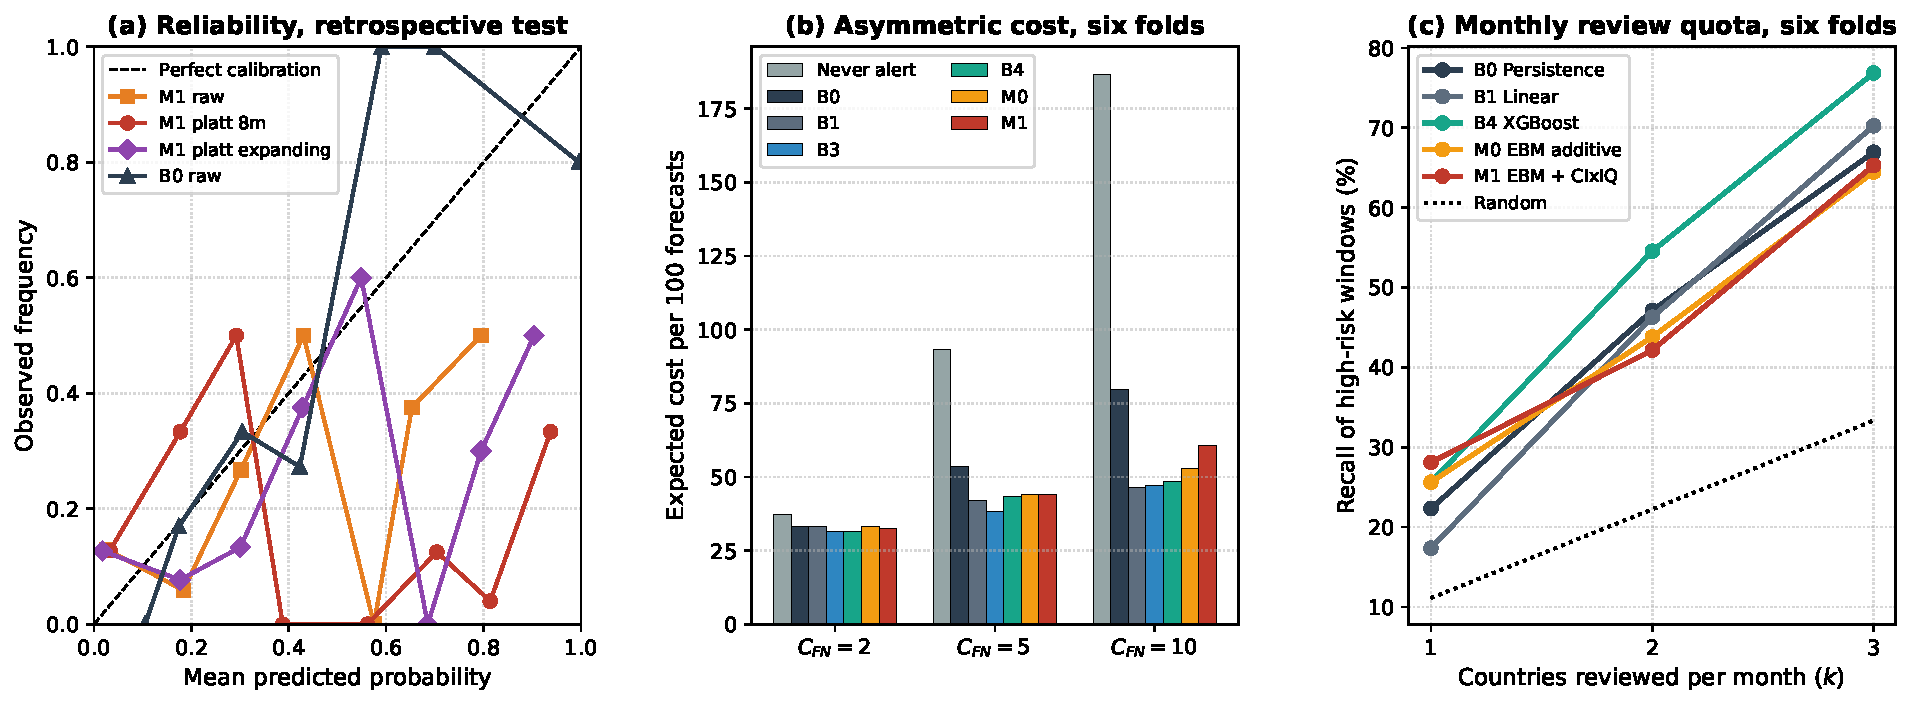
\includegraphics[width=\textwidth]{figures/Fig6.pdf}\caption{Reliability of M1 under three calibration schemes and of B0 in the retrospective test (a), expected cost under asymmetric losses over six folds (b) and recall under monthly review quotas over six folds (c).}\label{fig:fig4}\end{figure*}
\begin{figure*}[!htbp]\centering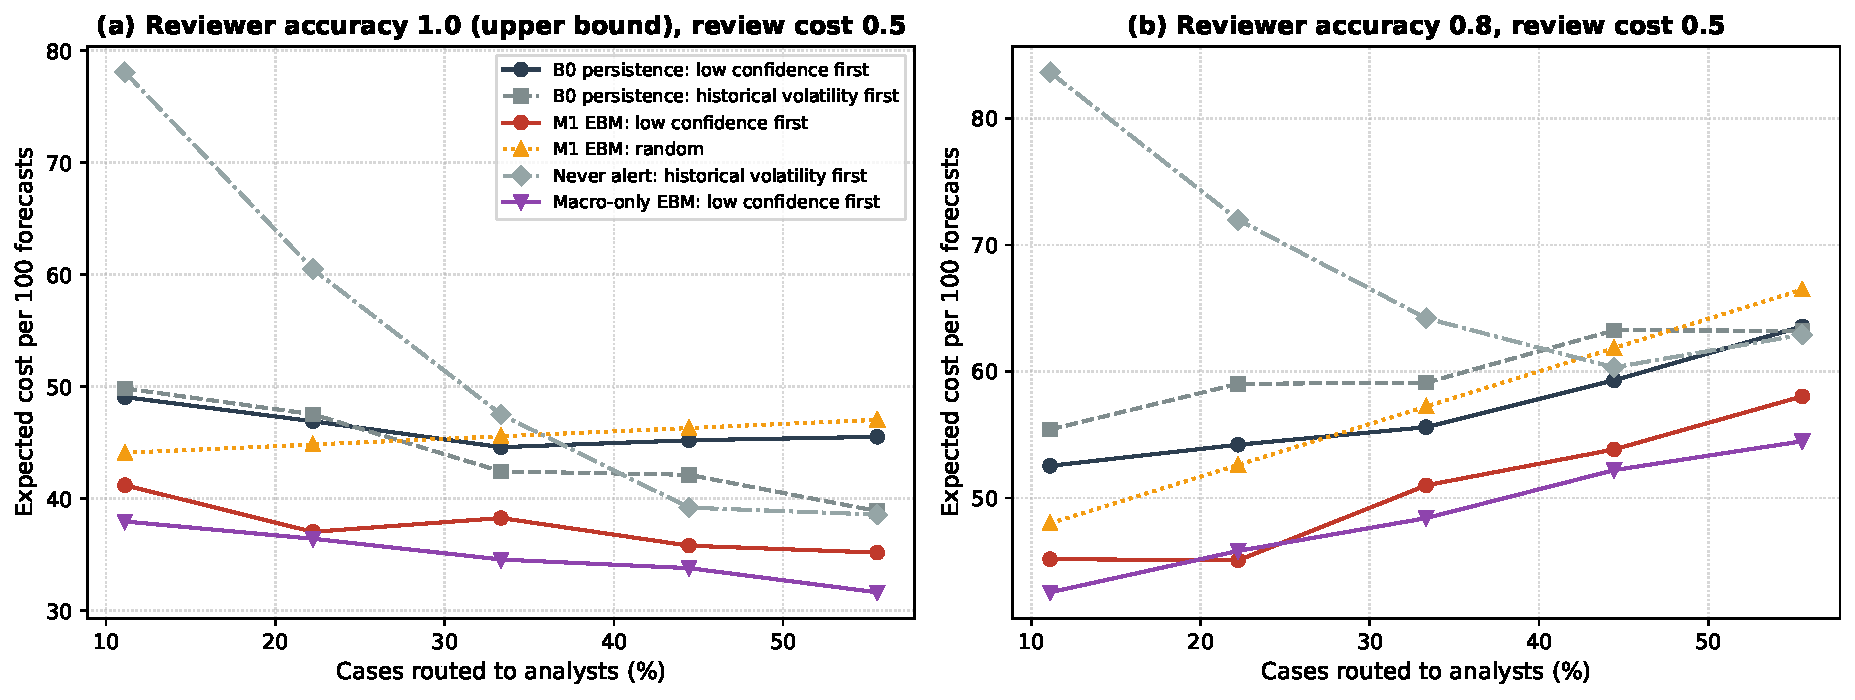
\includegraphics[width=\textwidth]{figures/Fig7.pdf}\caption{Expected cost against the share of cases reviewed (six folds, review fee 0.5) for selected automated policies and routing rules, with reviewer accuracy 1.0 (a, upper bound) and 0.8 (b).}\label{fig:fig7}\end{figure*}
\subsection{Robustness and information timing}
The reported EBM results are sensitive to information timing. Using month-$t$ REER values, which are not published at the end of month $t$, raises the pooled AP of M1 from 0.382 to 0.472 and of M0 from 0.388 to 0.462; an evaluation without the one-month REER lag would therefore overstate the EBMs' skill. Under longer assumed CI release lags of 3, 6 and 12 months M1 reaches 0.402, 0.375 and 0.396 over six folds, and freezing CI at the training cut-off gives 0.369. Other variations (Supplementary Table S6) change model rankings: with a q75 threshold B0, XGBoost and M1 reach 0.541, 0.583 and 0.522; with q90 (70 high-risk windows) 0.150, 0.227 and 0.271; with country-specific q80 thresholds 0.248, 0.393 and 0.381; at a six-month horizon 0.493, 0.438 and 0.386. Single WGI dimensions give M1 an AP between 0.359 and 0.385. Under leave-one-country-out validation the equal-weighted AP is 0.414 for B0 and 0.413 for M1, and deleting any single country moves the M1-M0 difference only between -0.013 and -0.001. Sub-period results, external transfer and adaptive training weights are reported in Supplementary Tables S7-S9.

Paired intervals qualify these comparisons. Of 26 model-versus-B0 contrasts across the robustness specifications, 6 favour the model with a 95\% interval above zero and none favours B0: B4 under Threshold q90 (pooled) (+0.077 [0.040, 0.182]); M0 under Threshold q90 (pooled) (+0.131 [0.059, 0.277]); M1 under Threshold q90 (pooled) (+0.121 [0.053, 0.267]); M0 under Threshold q80 (country-specific) (+0.130 [0.007, 0.219]); M1 under Threshold q80 (country-specific) (+0.133 [0.009, 0.216]); B4 under Reserve drawdown target (h=3) (+0.055 [0.005, 0.128]). Learned models thus beat persistence for rarer events, for country-specific thresholds, under which persistence is weak, and, for XGBoost, for the reserve target. In the matched Core-6 sample (84 high-risk windows in 432 country-months) M1 reaches 0.420 with SWIFT features and 0.398 without CI, a difference of 0.023 [-0.074, 0.082]; only 1 of 9 Core-6 CI comparisons excludes zero (both CI measures in B1, 0.029 [0.002, 0.094]). The main FX-share ablations do not show a 0.02 AP gain, but this result should not be generalized to every CI measure or risk definition.

\subsection{Frozen retrospective extension, 2023-2025}
Table~\ref{tab:confirm} reports the extension (84 high-risk windows in 540 country-months). The fallback rule deployed B0 in every year (2023: B0, 2024: B0, 2025: B0), so its cost equals that of B0, 53.7 per 100 forecasts against 77.8 for never alerting. Ex post, XGBoost had the highest AP (0.437 against 0.383 for B0) and a lower cost (41.7), but the cost difference is not significant (-12.0 [-31.1, 2.4]). In the Core-9 countries the AP gain of always using XGBoost over the fallback is 0.168 [0.066, 0.312], a gain the rule could not capture because it monitored the macro EBM; always using the macro EBM gives 0.024 [-0.158, 0.349]. In the six external economies B0 has the higher AP (0.433 against 0.311), whereas XGBoost has the lower simulated cost (48.1 versus 55.1), illustrating the distinction between ranking and decisions at a fixed threshold. Because the fallback equalled B0 in every year, it did not improve on always using B0; its value in this period is limited to having avoided the weaker macro EBM and B1.

\begin{table*}[!htbp]
\centering
\scriptsize
\setlength{\tabcolsep}{3pt}
\caption{Retrospective extension, forecast origins 2023-2025.}
\label{tab:confirm}
\par\smallskip{\textit{Panel A. Frozen protocol (macro and IQ features; scored once)}}\par\smallskip
\begin{adjustbox}{max width=\textwidth}
\begin{tabular}{llrrrrr}
\toprule
Model & AP (15) & Cost (15) & AP (Core-9) & Cost (Core-9) & AP (External-6) & Cost (External-6) \\
\midrule
Never alert &  & 77.8 &  & 72.5 &  & 85.6 \\
B0 Persistence & 0.383 & 53.7 & 0.378 & 52.8 & 0.433 & 55.1 \\
B1 Ridge / logistic & 0.261 & 55.4 & 0.412 & 42.6 & 0.221 & 74.5 \\
M0 EBM additive & 0.301 & 49.1 & 0.401 & 40.4 & 0.229 & 62.0 \\
B4 XGBoost & 0.437 & 41.7 & 0.545 & 37.3 & 0.311 & 48.1 \\
Fallback policy & 0.383 & 53.7 & 0.378 & 52.8 & 0.433 & 55.1 \\
\bottomrule
\end{tabular}
\end{adjustbox}
\par\smallskip{\textit{Panel B. Post-hoc rerun with corrected tuning (exploratory)}}\par\smallskip
\begin{adjustbox}{max width=\textwidth}
\begin{tabular}{llrrrrr}
\toprule
Model & AP (15) & Cost (15) & AP (Core-9) & Cost (Core-9) & AP (External-6) & Cost (External-6) \\
\midrule
B0 Persistence & 0.383 & 53.7 & 0.378 & 52.8 & 0.433 & 55.1 \\
C1 Country + persistence & 0.340 & 45.9 & 0.368 & 39.2 & 0.338 & 56.0 \\
B1 Ridge / logistic & 0.271 & 55.4 & 0.414 & 42.6 & 0.244 & 74.5 \\
Macro EBM (macro only) & 0.295 & 46.1 & 0.386 & 41.0 & 0.246 & 53.7 \\
Macro EBM (macro + IQ) & 0.324 & 45.7 & 0.425 & 39.8 & 0.271 & 54.6 \\
B4 XGBoost (macro only) & 0.422 & 41.9 & 0.542 & 36.7 & 0.312 & 49.5 \\
B4 XGBoost (macro + IQ) & 0.411 & 42.4 & 0.545 & 38.0 & 0.282 & 49.1 \\
Fallback rule, refitted & 0.383 & 53.7 & 0.378 & 52.8 & 0.433 & 55.1 \\
Multi-candidate monitor (exploratory) & 0.383 & 54.3 & 0.451 & 55.2 & 0.340 & 52.8 \\
\bottomrule
\end{tabular}
\end{adjustbox}
\par\vspace{2pt}\parbox{0.95\linewidth}{\scriptsize Note: 84 high-risk windows in 540 country-months (47 Core-9, 37 External-6). Pooled AP; cost per 100 forecasts at C\_FN = 5; raw probabilities. All models are trained on the pooled 15-country history. Frozen fallback deployments: 2023: B0, 2024: B0, 2025: B0; refitted fallback: 2023: B0, 2024: B0, 2025: B0; monitor: 2023: B0, 2024: B0, 2025: B4. Protocol SHA-256: 910490582b8dc40cfef8880dfcbc67bfa0786ea3867fead9de8d8ccf3718f65d.}
\end{table*}
\subsection{Post-hoc rerun of 2023-2025 with corrected tuning}
The post-hoc rerun (lower panel of Table~\ref{tab:confirm} and Table~\ref{tab:posthoc}) is exploratory. With the corrected tuning, adding IQ to the macro EBM raises pooled AP by 0.029 [0.002, 0.042] over the 15 countries, 0.039 [-0.010, 0.054] in Core-9 and 0.025 [0.001, 0.042] in External-6, while for XGBoost the increment is -0.011 [-0.040, 0.016]. The EBM gain also lowers the Brier score (-0.004 [-0.007, -0.000]) but not the expected cost (-0.4 [-3.3, 2.6]). IQ therefore adds ranking information to the additive model in this later period, of about the size of the chosen margin, but not to the stronger XGBoost model, and the macro+IQ EBM (0.324) remains below B0 (0.383). The refitted fallback rule again deploys B0 in every year: the AP gain of the macro EBM over B0 on the latest matured origins is 2023: -0.275, 2024: -0.243, 2025: -0.022. The exploratory multi-candidate monitor deploys 2023: B0, 2024: B0, 2025: B4. It ties with B0 over the 15 countries (0.000 [-0.029, 0.057]) and recovers part of the Core-9 gain (0.073 [0.000, 0.164]), but stays below always using XGBoost there (-0.094 [-0.276, 0.037]), because recent history favoured B0 until 2025 (recent AP of B0: 2023: 0.701, 2024: 0.661, 2025: 0.390; of XGBoost: 2023: 0.671, 2024: 0.557, 2025: 0.485). A monitored fallback reacts with a lag of at least one year to a change in model ranking.

\begin{table}[!htbp]
\centering
\scriptsize
\setlength{\tabcolsep}{3pt}
\caption{Post-hoc paired comparisons for 2023-2025 (A - B with 95\% block-bootstrap intervals).}
\label{tab:posthoc}
\begin{tabular}{lllrr}
\toprule
Comparison & Delta AP (15) & Delta AP (Core-9) & Delta AP (External-6) & Delta cost (15) \\
\midrule
Macro EBM: +IQ vs macro only & +0.029 [0.002, 0.042] & +0.039 [-0.010, 0.054] & +0.025 [0.001, 0.042] & -0.4 [-3.3, 2.6] \\
XGBoost: +IQ vs macro only & -0.011 [-0.040, 0.016] & +0.002 [-0.021, 0.022] & -0.030 [-0.045, 0.002] & +0.6 [-0.9, 2.8] \\
XGBoost vs B0 & +0.028 [-0.033, 0.142] & +0.167 [0.064, 0.317] & -0.151 [-0.316, 0.016] & -11.3 [-27.6, 3.3] \\
Macro+IQ EBM vs B0 & -0.059 [-0.139, 0.120] & +0.048 [-0.082, 0.281] & -0.162 [-0.329, 0.027] & -8.0 [-25.7, 12.6] \\
C1 vs B0 & -0.043 [-0.110, 0.056] & -0.010 [-0.071, 0.088] & -0.096 [-0.285, 0.069] & -7.8 [-27.8, 13.1] \\
Always XGBoost vs frozen fallback & +0.054 [-0.005, 0.175] & +0.168 [0.066, 0.312] & -0.122 [-0.309, 0.025] & -12.0 [-29.6, 3.3] \\
Always macro EBM vs frozen fallback & -0.082 [-0.197, 0.163] & +0.024 [-0.158, 0.349] & -0.205 [-0.352, -0.013] & -4.6 [-23.3, 17.8] \\
Always B1 vs frozen fallback & -0.122 [-0.239, 0.139] & +0.034 [-0.149, 0.380] & -0.212 [-0.367, 0.062] & +1.7 [-21.9, 31.1] \\
Monitor vs B0 & +0.000 [-0.029, 0.057] & +0.073 [0.000, 0.164] & -0.094 [-0.220, 0.005] & +0.6 [-6.1, 4.1] \\
Monitor vs XGBoost & -0.027 [-0.124, 0.052] & -0.094 [-0.276, 0.037] & +0.057 [-0.039, 0.191] & +11.9 [-2.8, 25.9] \\
\bottomrule
\end{tabular}
\par\vspace{2pt}\parbox{0.95\linewidth}{\scriptsize Note: Rows 1-5 and 9-10 use the post-hoc predictions with corrected tuning; rows 6-8 use the frozen predictions (the frozen fallback deployed B0 in every year, so always-B0 versus the fallback is identically zero). Moving-block bootstrap over months, L = 6, 1,000 replications. Brier differences and yearly fallback inputs are in the replication package (table15e, table15f).}
\end{table}
\section{Discussion}
\subsection{Decision rules}
Table~\ref{tab:rules} translates the results into conditional design considerations. Persistence and country-identity models provide useful reference points, while release assumptions, probability calibration and decision costs influence the evaluation. The CI-by-IQ interaction does not provide the chosen AP gain in the main comparison, and neither CI nor IQ does in the main FX-share ablations, but the paired intervals, the sensitivity results and the post-hoc IQ increment for the EBM prevent a blanket rejection of institutional or CI information. The policy results answer RQ3 comparatively: no evaluated decision rule is uniformly best across periods and assumptions.

\begin{table*}[!htbp]
\centering
\scriptsize
\setlength{\tabcolsep}{3pt}
\caption{Conditional design considerations derived from the reported evaluation.}
\label{tab:rules}
\begin{adjustbox}{max width=\textwidth}
\begin{tabular}{p{0.16\linewidth}p{0.38\linewidth}p{0.38\linewidth}}
\toprule
Decision & Rule & Evidence \\
\midrule
Feature set & Evaluate incremental CI and IQ information against a matched macro baseline with paired intervals & Main FX-share ablations: no gain of 0.02; 9 of 18 intervals cannot exclude one; post-hoc 2023-2025 IQ gain for the EBM 0.029 [0.002, 0.042] \\
Interaction & Validate the CI-by-IQ term before retaining it & M1 - M0: -0.005 [-0.029, 0.021]; equivalence within +/-0.02 not established \\
Benchmarks & Include persistence and country identity plus persistence & Retrospective AP: C1 0.574; B0 0.535; highest other multivariable AP 0.478 \\
Timing & Document release assumptions; enforce the maturity condition in every nested tuning and calibration stage & Using month-t REER changes M1 AP from 0.382 to 0.472; 452 audited numbers changed after the inner-fold correction \\
Calibration & Select calibration using earlier out-of-sample predictions relabelled to the current event & Eight-month Platt worsens Brier in 7 of 7 models \\
Analyst review & Compare routing rules under explicit reviewer-error and fee assumptions with matched budgets & LC vs random (oracle review): -6.9 [-14.5, -2.1]; with imperfect reviewers review never beats no review significantly \\
Fallback & Evaluate the opportunity cost of the monitored candidate set, not only protection against weak models & Frozen rule retains B0 throughout; always XGBoost in Core-9: 0.168 [0.066, 0.312] AP \\
\bottomrule
\end{tabular}
\end{adjustbox}
\par\vspace{2pt}\parbox{0.95\linewidth}{\scriptsize Note: Numbers are pooled over six folds unless stated; intervals are 95\% paired block-bootstrap intervals.}
\end{table*}
\subsection{Implications for expert and decision-support systems}
The applied contribution is an audit workflow for moving from regression-based motivation to a predictive decision-support task. First, an in-sample association does not establish forecasting value. Second, the reported EBM estimates change materially when the REER availability assumption changes; publication timing is therefore part of the model specification, and the timing condition must hold in every nested stage, not only at the outer test boundary, as the corrections in Section 4.5 illustrate. Third, ranking quality, probability quality and decision cost are separate criteria: a model may lead on one and not another. Fourth, decision rules that rely on model probabilities, such as expected-loss routing, inherit their calibration errors. Fifth, the later evaluation reveals a limitation of a single-candidate fallback: it can retain a competitive baseline while missing improvement from a different candidate, and monitoring several candidates reacts only after the ranking has changed. These findings motivate transparent validation and monitoring. They do not establish a new optimal learning algorithm or demonstrate the effectiveness of a deployed early-warning service.

\subsection{Limitations}
The primary forecasting panel contains nine countries over eleven years, with 31 labelled episodes in the evaluated folds. Overlapping targets, common shocks and the limited number of country clusters constrain inference; short evaluation windows yield few independent time blocks, and half of the ablation intervals are too wide to exclude a gain of the chosen size. Development-period model selection and retrospective inspection of 2021-2022 limit claims of untouched testing. The 2023-2025 extension is historical, uses a frozen protocol with an analysis history that includes prior target-summary inspection and a tuning error corrected after scoring, and cannot test updated CI; its IQ ablation is post hoc. The data are release-lag adjusted rather than fully vintage reconstructed; current-vintage revisions and uncertain source calendars remain limitations. The Wind CI construction could not be re-verified, and changing a nominal lag does not resolve provenance or measurement validity. The replication preserves a dynamic fixed-effects specification, so Nickell bias \citep{nickell1981} and the applicability of non-dynamic threshold-test inference require caution; the country-block bootstrap holds the lagged dependent variable fixed and rests on six or nine resampling units. A search for specifications that reproduce earlier tables is not an independent hypothesis test. The policy simulation assumes costs and reviewer-error mechanisms; it is neither a field trial nor evidence that real analysts can achieve the simulated gains. AP equivalence is local to a stated margin and comparison, and is not evidence of economic equivalence or policy causality.

\section{Conclusion}
This study evaluates whether institution-conditioned currency-internationalization evidence can inform exchange-rate stress prediction and decision support. A compatible calculation reproduces the reported threshold tests, but several results are sensitive to trimming and model assumptions. In the main FX-share forecasting comparisons, CI and IQ additions do not achieve the chosen 0.02 AP gain, but the paired intervals are often too wide to exclude it, and interaction equivalence is not established. Alternative CI measures, stress thresholds and later country samples yield heterogeneous results, including a post-hoc IQ gain for the additive model in 2023-2025. The retrospective extension evaluates model and fallback performance rather than confirming a null contribution from CI or IQ; its single-candidate fallback retains persistence in every year and misses the core-sample improvement from XGBoost. The practical contribution is a transparent audit workflow that separates reproducibility, predictive value and simulated decision value, checks the timing of every estimation stage and makes the limits of the evidence explicit before deployment.

\section*{Data availability}
BIS, IMF and World Bank data are public; the Wind-based regression datasets (compiled on 13 June 2023) are licensed and cannot be redistributed, but their variables are documented in Supplementary Table S15 and their SHA-256 checksums are included in the replication package. Code, split definitions, the frozen protocol and its change log, the timing audit, all row-level predictions with labels, the archived first-draft outputs and a single entry script (run\_all.sh) are provided as an anonymized reproduction archive submitted with the manuscript (MacroRisk\_reproduction\_anonymized.zip) and at an anonymous read-only mirror [anonymous mirror link to be inserted before submission].
\begin{thebibliography}{99}
\bibitem[Aman et~al.(2024)]{aman2024} Aman, Z., Granville, B., Mallick, S. K., \& Nemlioglu, I. (2024). Does greater financial openness promote external competitiveness in emerging markets? The role of institutional quality. International Journal of Finance \& Economics, 29(1), 486-510. https://doi.org/10.1002/ijfe.2695
\bibitem[An et~al.(2024)]{an2024} An, J., Kim, H. S., \& Park, B. (2024). Do China's policy measures for RMB internationalization foster currency co-movements? International Review of Economics \& Finance, 91, 1033-1050. https://doi.org/10.1016/j.iref.2024.01.019
\bibitem[Barthélémy et~al.(2024)]{barthelemy2024} Barthélémy, S., Gautier, V., \& Rondeau, F. (2024). Early warning system for currency crises using long short-term memory and gated recurrent unit neural networks. Journal of Forecasting, 43(5), 1235-1262. https://doi.org/10.1002/for.3069
\bibitem[Beutel et~al.(2019)]{beutel2019} Beutel, J., List, S., \& von Schweinitz, G. (2019). Does machine learning help us predict banking crises? Journal of Financial Stability, 45, 100693. https://doi.org/10.1016/j.jfs.2019.100693
\bibitem[Bluwstein et~al.(2023)]{bluwstein2023} Bluwstein, K., Buckmann, M., Joseph, A., Kapadia, S., \& Simsek, O. (2023). Credit growth, the yield curve and financial crisis prediction: Evidence from a machine learning approach. Journal of International Economics, 145, 103773. https://doi.org/10.1016/j.jinteco.2023.103773
\bibitem[Breiman(2001)]{breiman2001} Breiman, L. (2001). Random forests. Machine Learning, 45(1), 5-32.
\bibitem[Chen et~al.(2024)]{chen2024} Chen, S., Huang, Y., \& Ge, L. (2024). An early warning system for financial crises: A temporal convolutional network approach. Technological and Economic Development of Economy, 30(3), 688-711. https://doi.org/10.3846/tede.2024.20555
\bibitem[Chen \& Guestrin(2016)]{chen2016} Chen, T., \& Guestrin, C. (2016). XGBoost: A scalable tree boosting system. In Proceedings of the 22nd ACM SIGKDD International Conference on Knowledge Discovery and Data Mining (pp. 785-794).
\bibitem[Chinn \& Ito(2006)]{chinn2006} Chinn, M. D., \& Ito, H. (2006). What matters for financial development? Capital controls, institutions, and interactions. Journal of Development Economics, 81(1), 163-192.
\bibitem[Chow(1970)]{chow1970} Chow, C. K. (1970). On optimum recognition error and reject tradeoff. IEEE Transactions on Information Theory, 16(1), 41-46.
\bibitem[Croushore \& Stark(2001)]{croushore2001} Croushore, D., \& Stark, T. (2001). A real-time data set for macroeconomists. Journal of Econometrics, 105(1), 111-130.
\bibitem[Davison \& Hinkley(1997)]{davison1997} Davison, A. C., \& Hinkley, D. V. (1997). Bootstrap methods and their application. Cambridge University Press.
\bibitem[Eichengreen et~al.(2018)]{eichengreen2018} Eichengreen, B., Mehl, A., \& Chitu, L. (2018). How global currencies work: Past, present, and future. Princeton University Press.
\bibitem[Elkan(2001)]{elkan2001} Elkan, C. (2001). The foundations of cost-sensitive learning. In Proceedings of the 17th International Joint Conference on Artificial Intelligence (pp. 973-978).
\bibitem[Frankel \& Rose(1996)]{frankel1996} Frankel, J. A., \& Rose, A. K. (1996). Currency crashes in emerging markets: An empirical treatment. Journal of International Economics, 41(3-4), 351-366.
\bibitem[Gama et~al.(2014)]{gama2014} Gama, J., Zliobaite, I., Bifet, A., Pechenizkiy, M., \& Bouchachia, A. (2014). A survey on concept drift adaptation. ACM Computing Surveys, 46(4), 44.
\bibitem[Geifman \& El-Yaniv(2017)]{geifman2017} Geifman, Y., \& El-Yaniv, R. (2017). Selective classification for deep neural networks. In Advances in Neural Information Processing Systems 30.
\bibitem[Hansen(1999)]{hansen1999} Hansen, B. E. (1999). Threshold effects in non-dynamic panels: Estimation, testing, and inference. Journal of Econometrics, 93(2), 345-368.
\bibitem[Holopainen \& Sarlin(2017)]{holopainen2017} Holopainen, M., \& Sarlin, P. (2017). Toward robust early-warning models: A horse race, ensembles and model uncertainty. Quantitative Finance, 17(12), 1933-1963.
\bibitem[Kaminsky et~al.(1998)]{kaminsky1998} Kaminsky, G., Lizondo, S., \& Reinhart, C. M. (1998). Leading indicators of currency crises. IMF Staff Papers, 45(1), 1-48.
\bibitem[Kaufmann et~al.(2011)]{kaufmann2011} Kaufmann, D., Kraay, A., \& Mastruzzi, M. (2011). The Worldwide Governance Indicators: Methodology and analytical issues. Hague Journal on the Rule of Law, 3(2), 220-246.
\bibitem[Kunsch(1989)]{kunsch1989} Kunsch, H. R. (1989). The jackknife and the bootstrap for general stationary observations. The Annals of Statistics, 17(3), 1217-1241.
\bibitem[Lakens(2017)]{lakens2017} Lakens, D. (2017). Equivalence tests: A practical primer for t tests, correlations, and meta-analyses. Social Psychological and Personality Science, 8(4), 355-362.
\bibitem[Lou et~al.(2012)]{lou2012} Lou, Y., Caruana, R., \& Gehrke, J. (2012). Intelligible models for classification and regression. In Proceedings of the 18th ACM SIGKDD International Conference on Knowledge Discovery and Data Mining (pp. 150-158).
\bibitem[Nickell(1981)]{nickell1981} Nickell, S. (1981). Biases in dynamic models with fixed effects. Econometrica, 49(6), 1417-1426.
\bibitem[Niculescu-Mizil \& Caruana(2005)]{niculescu2005} Niculescu-Mizil, A., \& Caruana, R. (2005). Predicting good probabilities with supervised learning. In Proceedings of the 22nd International Conference on Machine Learning (pp. 625-632).
\bibitem[Nori et~al.(2019)]{nori2019} Nori, H., Jenkins, S., Koch, P., \& Caruana, R. (2019). InterpretML: A unified framework for machine learning interpretability. arXiv preprint arXiv:1909.09223.
\bibitem[Ostrensky \& Frota(2023)]{ostrensky2023} Ostrensky, V. P., \& Frota, L. M. da (2023). Early warning systems via machine learning: A study of currency crises. Economia Aplicada, 27(3), 407-423. https://doi.org/10.11606/1980-5330/ea189768
\bibitem[Platt(1999)]{platt1999} Platt, J. (1999). Probabilistic outputs for support vector machines and comparisons to regularized likelihood methods. In Advances in Large Margin Classifiers (pp. 61-74). MIT Press.
\bibitem[Reimann(2024)]{reimann2024} Reimann, C. (2024). Predicting financial crises: An evaluation of machine learning algorithms and model explainability for early warning systems. Review of Evolutionary Political Economy, 5(1), 51-83. https://doi.org/10.1007/s43253-024-00114-4
\bibitem[Rudin(2019)]{rudin2019} Rudin, C. (2019). Stop explaining black box machine learning models for high stakes decisions and use interpretable models instead. Nature Machine Intelligence, 1(5), 206-215.
\bibitem[Saito \& Rehmsmeier(2015)]{saito2015} Saito, T., \& Rehmsmeier, M. (2015). The precision-recall plot is more informative than the ROC plot when evaluating binary classifiers on imbalanced datasets. PLoS ONE, 10(3), e0118432.
\bibitem[Schuirmann(1987)]{schuirmann1987} Schuirmann, D. J. (1987). A comparison of the two one-sided tests procedure and the power approach for assessing the equivalence of average bioavailability. Journal of Pharmacokinetics and Biopharmaceutics, 15(6), 657-680.
\bibitem[Wang(2015)]{wang2015} Wang, Q. (2015). Fixed-effect panel threshold model using Stata. The Stata Journal, 15(1), 121-134.
\end{thebibliography}
\end{document}